\KOMAoption{paper}{a4, portrait}
\areaset{267mm}{180mm}
\fancyheadoffset{0pt} % обновляем хедер и футер

\newgeometry{
  top=14mm,
  bottom=11mm,
  right=10mm,
  left=22mm,
}

\begin{landscape}

%\setlength{\headsep}{5.6mm} 
%\setlength{\topmargin}{-27mm}
\setlength{\footskip}{15.5pt}
%\setlength{\textwidth}{305mm}

\color{uniblue}{\section[(справочное) Перечень сигналов ФСУ, предназначенных \newline для конфигурирования устройства <<ЮНИТ-М300-ОЛ>>]{(справочное)\\Перечень сигналов ФСУ, предназначенных для конфигурирования устройства <<ЮНИТ-М300-ОЛ>>}\label{app:signals}}
\color{black}

\begin{enumerate}[label=\ref{app:signals}.\arabic*] % Без глобального влияния
  \item Перечень сигналов самодиагностики, доступных для конфигурирования, приведен в документации ЮТКБ.656122.609 РЭ <<Устройство защиты и автоматики серии <<ЮНИТ-М300>>. Руководство по эксплуатации общее>>.
  \item Условные обозначения, применяемые в таблице перечня сигналов:
  \begin{itemize}
    \item[$\text{(--)}$] { - сигнал не имеет возможности конфигурации;}
    \item[$\text{(+)}$] { - сигнал имеет возможность конфигурации;}
    \item[$\text{(*)}$] { - конфигурация сигнала предустановлена по умолчанию в сервисном ПО <<ЮНИТ-СЕРВИС>> и не может быть изменена.}
  \end{itemize}
\end{enumerate}

\small % сделаем шрифт в таблице поменьше
% В таблице ниже убрал правую и левую горизонтальные линии чтобы не сливались и жирно видно - также в настройках geometry прищлось поле right =8mm а не 5 mm 
% так как строки ниже колонтитулов спускались
\begin{longtable}{
>{\centering\arraybackslash}m{6.0cm}
|>{\centering\arraybackslash}m{3.45cm}
|>{\centering\arraybackslash}m{2cm}
|>{\centering\arraybackslash}m{2cm}
|>{\centering\arraybackslash}m{2cm}
|>{\centering\arraybackslash}m{2cm}
|>{\centering\arraybackslash}m{2cm}
|>{\centering\arraybackslash}m{2cm}
|>{\centering\arraybackslash}m{2.107cm}
}

%\caption{Перечень сигналов ФСУ, предназначенных для конфигурирования устройств ЮНИТ-М300\vspace{-0.5\baselineskip}}\label{appA:tbl1}\\ % выравнивает надпись посередине таблицы
\caption{Перечень сигналов ФСУ, предназначенных для конфигурирования устройства\hfill\vspace{-0.5\baselineskip}}\label{appA:tbl1}\\ 

\hline
\rowcolor{gray!30}
Полное наименование сигнала & Наименование сигнала на ФСУ & Дискретные входы & Выходные реле & Светодиоды & Функционал. клавиши & Регистратор событий & Аварийный осциллограф & Пуск авар. осциллографа \\ 
\hline
\endfirsthead
%\caption{\emph{Продолжение\vspace{-0.5\baselineskip}}} \\ % Отступ обозначения таблицы от таблицы и выравнивание надписи слева
\caption*{\hspace{3pt}\emph{Продолжение таблицы \ref{appA:tbl1}\hfill\vspace{-0.5\baselineskip}}} \\ % сделано по ГОСТ 2.105 п.6.8.7
\hline
\rowcolor{gray!30}
Полное наименование сигнала & Наименование сигнала на ФСУ & Дискретные входы & Выходные реле & Светодиоды & Функционал. клавиши & Регистратор событий & Аварийный осциллограф & Пуск авар. осциллографа \\ 
%\hline
\endhead

%\hline
\endfoot

%\hline
\endlastfoot

%===t2
\multicolumn{9}{c}{\textbf{Виртуальные ключи}} \\
\hline
\raggedright Вывод терминала & \centering Вывод терминала & \centering -- & \centering -- & \centering -- & \centering + & \centering + & \centering + & \centering \arraybackslash + \\ \hline
\raggedright Оперативный вывод функции ДЗ & \centering ОВ ДЗ & \centering -- & \centering -- & \centering -- & \centering + & \centering + & \centering + & \centering \arraybackslash + \\ \hline
\raggedright Оперативный вывод 1 ступени ДЗ-фф & \centering ОВ ДЗ-фф 1ст. & \centering -- & \centering -- & \centering -- & \centering + & \centering + & \centering + & \centering \arraybackslash + \\ \hline
\raggedright Перевод 1 ступени ДЗ-фф на сигнал & \centering ДЗ-фф 1ст. на сигн & \centering -- & \centering -- & \centering -- & \centering + & \centering + & \centering + & \centering \arraybackslash + \\ \hline
\raggedright Оперативный вывод 2 ступени ДЗ-фф & \centering ОВ ДЗ-фф 2ст. & \centering -- & \centering -- & \centering -- & \centering + & \centering + & \centering + & \centering \arraybackslash + \\ \hline
\raggedright Перевод 2 ступени ДЗ-фф на сигнал & \centering ДЗ-фф 2ст. на сигн & \centering -- & \centering -- & \centering -- & \centering + & \centering + & \centering + & \centering \arraybackslash + \\ \hline
\raggedright Оперативный вывод 3 ступени ДЗ-фф & \centering ОВ ДЗ-фф 3ст. & \centering -- & \centering -- & \centering -- & \centering + & \centering + & \centering + & \centering \arraybackslash + \\ \hline
\raggedright Перевод 3 ступени ДЗ-фф на сигнал & \centering ДЗ-фф 3ст. на сигн & \centering -- & \centering -- & \centering -- & \centering + & \centering + & \centering + & \centering \arraybackslash + \\ \hline
\raggedright Оперативный вывод 4 ступени ДЗ-фф & \centering ОВ ДЗ-фф 4ст. & \centering -- & \centering -- & \centering -- & \centering + & \centering + & \centering + & \centering \arraybackslash + \\ \hline
\raggedright Перевод 4 ступени ДЗ-фф на сигнал & \centering ДЗ-фф 4ст. на сигн & \centering -- & \centering -- & \centering -- & \centering + & \centering + & \centering + & \centering \arraybackslash + \\ \hline
\raggedright Сигнал ввода оперативного ускорения ДЗ & \centering Ввод ОУ ДЗ & \centering -- & \centering -- & \centering -- & \centering + & \centering + & \centering + & \centering \arraybackslash + \\ \hline
\raggedright Оперативный вывод функции БК & \centering ОВ БК & \centering -- & \centering -- & \centering -- & \centering + & \centering + & \centering + & \centering \arraybackslash + \\ \hline
\raggedright Оперативный вывод функции МТЗ & \centering ОВ МТЗ & \centering -- & \centering -- & \centering -- & \centering + & \centering + & \centering + & \centering \arraybackslash + \\ \hline
\raggedright Сигнал ввода оперативного ускорения МТЗ & \centering Ввод ОУ МТЗ & \centering -- & \centering -- & \centering -- & \centering + & \centering + & \centering + & \centering \arraybackslash + \\ \hline
\raggedright Оперативный вывод 1 ступени МТЗ & \centering ОВ МТЗ 1 ст. & \centering -- & \centering -- & \centering -- & \centering + & \centering + & \centering + & \centering \arraybackslash + \\ \hline
\raggedright Перевод МТЗ 1 ступени на сигнал & \centering МТЗ 1ст. на сигн & \centering -- & \centering -- & \centering -- & \centering + & \centering + & \centering + & \centering \arraybackslash + \\ \hline
\raggedright Оперативный вывод 2 ступени МТЗ & \centering ОВ МТЗ 2 ст. & \centering -- & \centering -- & \centering -- & \centering + & \centering + & \centering + & \centering \arraybackslash + \\ \hline
\raggedright Перевод МТЗ 2 ступени на сигнал & \centering МТЗ 2ст. на сигн & \centering -- & \centering -- & \centering -- & \centering + & \centering + & \centering + & \centering \arraybackslash + \\ \hline
\raggedright Оперативный вывод 3 ступени МТЗ & \centering ОВ МТЗ 3 ст. & \centering -- & \centering -- & \centering -- & \centering + & \centering + & \centering + & \centering \arraybackslash + \\ \hline
\raggedright Перевод МТЗ 3 ступени на сигнал & \centering МТЗ 3ст. на сигн & \centering -- & \centering -- & \centering -- & \centering + & \centering + & \centering + & \centering \arraybackslash + \\ \hline
\raggedright Оперативный вывод 4 ступени МТЗ & \centering ОВ МТЗ 4 ст. & \centering -- & \centering -- & \centering -- & \centering + & \centering + & \centering + & \centering \arraybackslash + \\ \hline
\raggedright Перевод МТЗ 4 ступени на сигнал & \centering МТЗ 4ст. на сигн & \centering -- & \centering -- & \centering -- & \centering + & \centering + & \centering + & \centering \arraybackslash + \\ \hline
\raggedright Оперативный вывод функции ЛЗШ & \centering ОВ ЛЗШ & \centering -- & \centering -- & \centering -- & \centering + & \centering + & \centering + & \centering \arraybackslash + \\ \hline
\raggedright Перевод ЛЗШ на сигнал & \centering ЛЗШ на сигн & \centering -- & \centering -- & \centering -- & \centering + & \centering + & \centering + & \centering \arraybackslash + \\ \hline
\raggedright Оперативный вывод функции ЗДЗ & \centering ОВ ЗДЗ & \centering -- & \centering -- & \centering -- & \centering + & \centering + & \centering + & \centering \arraybackslash + \\ \hline
\raggedright Перевод ЗДЗ на сигнал & \centering ЗДЗ на сигн & \centering -- & \centering -- & \centering -- & \centering + & \centering + & \centering + & \centering \arraybackslash + \\ \hline
\raggedright Оперативный вывод функции ТК ЗДЗ & \centering ОВ ТК ЗДЗ & \centering -- & \centering -- & \centering -- & \centering + & \centering + & \centering + & \centering \arraybackslash + \\ \hline
\raggedright Оперативный вывод функции ЗОП & \centering ОВ ЗОП & \centering -- & \centering -- & \centering -- & \centering + & \centering + & \centering + & \centering \arraybackslash + \\ \hline
\raggedright Перевод ЗОП на сигнал & \centering ЗОП на сигн & \centering -- & \centering -- & \centering -- & \centering + & \centering + & \centering + & \centering \arraybackslash + \\ \hline
\raggedright Оперативный вывод функции ТЗНП & \centering ОВ ТЗНП & \centering -- & \centering -- & \centering -- & \centering + & \centering + & \centering + & \centering \arraybackslash + \\ \hline
\raggedright Режим работы ЧС & \centering Режим работы ЧС & \centering -- & \centering -- & \centering -- & \centering + & \centering + & \centering + & \centering \arraybackslash + \\ \hline
\raggedright Перевод ТЗНП 1 ступени на сигнал & \centering ТЗНП 1ст. на сигн & \centering -- & \centering -- & \centering -- & \centering + & \centering + & \centering + & \centering \arraybackslash + \\ \hline
\raggedright Перевод ТЗНП 2 ступени на сигнал & \centering ТЗНП 2ст. на сигн & \centering -- & \centering -- & \centering -- & \centering + & \centering + & \centering + & \centering \arraybackslash + \\ \hline
\raggedright Перевод ТЗНП 3 ступени на сигнал & \centering ТЗНП 3ст. на сигн & \centering -- & \centering -- & \centering -- & \centering + & \centering + & \centering + & \centering \arraybackslash + \\ \hline
\raggedright Перевод ТЗНП 4 ступени на сигнал & \centering ТЗНП 4ст. на сигн & \centering -- & \centering -- & \centering -- & \centering + & \centering + & \centering + & \centering \arraybackslash + \\ \hline
\raggedright Сигнал ввода оперативного ускорения ТЗНП & \centering Ввод ОУ ТЗНП & \centering -- & \centering -- & \centering -- & \centering + & \centering + & \centering + & \centering \arraybackslash + \\ \hline
\raggedright Оперативный вывод функции УРОВ & \centering ОВ УРОВ & \centering -- & \centering -- & \centering -- & \centering + & \centering + & \centering + & \centering \arraybackslash + \\ \hline
\raggedright Оперативный вывод функции БНН 1 секции шин & \centering ОВ БНН 1сш & \centering -- & \centering -- & \centering -- & \centering + & \centering + & \centering + & \centering \arraybackslash + \\ \hline
\raggedright Фиксация неисправности цепей напряжения шин & \centering Фикс.неисп.ЦНш & \centering -- & \centering -- & \centering -- & \centering + & \centering + & \centering + & \centering \arraybackslash + \\ \hline
\raggedright Оперативный вывод функции БНН 2 секции шин & \centering ОВ БНН 2сш & \centering -- & \centering -- & \centering -- & \centering + & \centering + & \centering + & \centering \arraybackslash + \\ \hline
\raggedright Оперативный вывод функции КНН 1 секции шин & \centering ОВ КНН 1сш & \centering -- & \centering -- & \centering -- & \centering + & \centering + & \centering + & \centering \arraybackslash + \\ \hline
\raggedright Оперативный вывод функции КНН 2 секции шин & \centering ОВ КНН 2сш & \centering -- & \centering -- & \centering -- & \centering + & \centering + & \centering + & \centering \arraybackslash + \\ \hline
\raggedright Оперативный вывод функции КОН 1 секции шин & \centering ОВ КОН 1сш & \centering -- & \centering -- & \centering -- & \centering + & \centering + & \centering + & \centering \arraybackslash + \\ \hline
\raggedright Оперативный вывод функции КОН 2 секции шин & \centering ОВ КОН 2сш & \centering -- & \centering -- & \centering -- & \centering + & \centering + & \centering + & \centering \arraybackslash + \\ \hline
\raggedright Оперативный вывод функции КС & \centering ОВ КС & \centering -- & \centering -- & \centering -- & \centering + & \centering + & \centering + & \centering \arraybackslash + \\ \hline
\raggedright Оперативный вывод функции АВР & \centering ОВ АВР & \centering -- & \centering -- & \centering -- & \centering + & \centering + & \centering + & \centering \arraybackslash + \\ \hline
\raggedright Оперативный вывод функции ВНР & \centering ОВ ВНР & \centering -- & \centering -- & \centering -- & \centering + & \centering + & \centering + & \centering \arraybackslash + \\ \hline
\multicolumn{9}{c}{\textbf{Общие сигналы функциональной логики}} \\
\hline
\rowcolor{gray!15} 
\multicolumn{9}{c}{Дистанционная защита (ДЗ)} \\
\hline
\multicolumn{9}{c}{1 ступень дистанционной защиты по контуру «фаза-фаза» (ДЗ-фф 1ст.)} \\
\hline
\raggedright  Функция введена в работу & \centering Ввод & \centering -- & \centering + & \centering + & \centering -- & \centering + & \centering + & \centering \arraybackslash + \\ \hline
\raggedright  Функция оперативно выведена из работы & \centering Оперативный вывод & \centering -- & \centering + & \centering + & \centering -- & \centering + & \centering + & \centering \arraybackslash + \\ \hline
\raggedright  Пуск ИО сопротивления Zab (фаза-фаза1) & \centering ИО Zab & \centering -- & \centering + & \centering + & \centering -- & \centering + & \centering + & \centering \arraybackslash + \\ \hline
\raggedright  Пуск ИО сопротивления Zbc (фаза-фаза1) & \centering ИО Zbc & \centering -- & \centering + & \centering + & \centering -- & \centering + & \centering + & \centering \arraybackslash + \\ \hline
\raggedright  Пуск ИО сопротивления Zca (фаза-фаза1) & \centering ИО Zca & \centering -- & \centering + & \centering + & \centering -- & \centering + & \centering + & \centering \arraybackslash + \\ \hline
\raggedright  Пуск ДЗ-фф 1 ст. & \centering Пуск & \centering -- & \centering + & \centering + & \centering -- & \centering + & \centering + & \centering \arraybackslash + \\ \hline
\raggedright  Срабатывание на сигнал & \centering Срабатывание сигн & \centering -- & \centering + & \centering + & \centering -- & \centering + & \centering + & \centering \arraybackslash + \\ \hline
\raggedright  Срабатывание ДЗ-фф 1 ст. & \centering Срабатывание & \centering -- & \centering + & \centering + & \centering -- & \centering + & \centering + & \centering \arraybackslash + \\ \hline
\multicolumn{9}{c}{2 ступень дистанционной защиты по контуру «фаза-фаза» (ДЗ-фф 2ст.)} \\
\hline
\raggedright  Функция введена в работу & \centering Ввод & \centering -- & \centering + & \centering + & \centering -- & \centering + & \centering + & \centering \arraybackslash + \\ \hline
\raggedright  Функция оперативно выведена из работы & \centering Оперативный вывод & \centering -- & \centering + & \centering + & \centering -- & \centering + & \centering + & \centering \arraybackslash + \\ \hline
\raggedright  Пуск ИО сопротивления Zab (фаза-фаза2) & \centering ИО Zab & \centering -- & \centering + & \centering + & \centering -- & \centering + & \centering + & \centering \arraybackslash + \\ \hline
\raggedright  Пуск ИО сопротивления Zbc (фаза-фаза2) & \centering ИО Zbc & \centering -- & \centering + & \centering + & \centering -- & \centering + & \centering + & \centering \arraybackslash + \\ \hline
\raggedright  Пуск ИО сопротивления Zca (фаза-фаза2) & \centering ИО Zca & \centering -- & \centering + & \centering + & \centering -- & \centering + & \centering + & \centering \arraybackslash + \\ \hline
\raggedright  Пуск ДЗ-фф 2 ст. & \centering Пуск & \centering -- & \centering + & \centering + & \centering -- & \centering + & \centering + & \centering \arraybackslash + \\ \hline
\raggedright  Срабатывание на сигнал & \centering Срабатывание сигн & \centering -- & \centering + & \centering + & \centering -- & \centering + & \centering + & \centering \arraybackslash + \\ \hline
\raggedright  Срабатывание ДЗ-фф 2 ст. & \centering Срабатывание & \centering -- & \centering + & \centering + & \centering -- & \centering + & \centering + & \centering \arraybackslash + \\ \hline
\multicolumn{9}{c}{3 ступень дистанционной защиты по контуру  «фаза-фаза» (ДЗ-фф 3ст.)} \\
\hline
\raggedright  Функция введена в работу & \centering Ввод & \centering -- & \centering + & \centering + & \centering -- & \centering + & \centering + & \centering \arraybackslash + \\ \hline
\raggedright  Функция оперативно выведена из работы & \centering Оперативный вывод & \centering -- & \centering + & \centering + & \centering -- & \centering + & \centering + & \centering \arraybackslash + \\ \hline
\raggedright  Пуск ИО сопротивления Zab (фаза-фаза3) & \centering ИО Zab & \centering -- & \centering + & \centering + & \centering -- & \centering + & \centering + & \centering \arraybackslash + \\ \hline
\raggedright  Пуск ИО сопротивления Zbc (фаза-фаза3) & \centering ИО Zbc & \centering -- & \centering + & \centering + & \centering -- & \centering + & \centering + & \centering \arraybackslash + \\ \hline
\raggedright  Пуск ИО сопротивления Zca (фаза-фаза3) & \centering ИО Zca & \centering -- & \centering + & \centering + & \centering -- & \centering + & \centering + & \centering \arraybackslash + \\ \hline
\raggedright  Пуск ДЗ-фф 3 ст. & \centering Пуск & \centering -- & \centering + & \centering + & \centering -- & \centering + & \centering + & \centering \arraybackslash + \\ \hline
\raggedright  Срабатывание на сигнал & \centering Срабатывание сигн & \centering -- & \centering + & \centering + & \centering -- & \centering + & \centering + & \centering \arraybackslash + \\ \hline
\raggedright  Срабатывание ДЗ-фф 3 ст. & \centering Срабатывание & \centering -- & \centering + & \centering + & \centering -- & \centering + & \centering + & \centering \arraybackslash + \\ \hline
\multicolumn{9}{c}{4 ступень дистанционной защиты по контуру «фаза-фаза» (ДЗ-фф 4ст.)} \\
\hline
\raggedright  Функция введена в работу & \centering Ввод & \centering -- & \centering + & \centering + & \centering -- & \centering + & \centering + & \centering \arraybackslash + \\ \hline
\raggedright  Функция оперативно выведена из работы & \centering Оперативный вывод & \centering -- & \centering + & \centering + & \centering -- & \centering + & \centering + & \centering \arraybackslash + \\ \hline
\raggedright  Пуск ИО сопротивления Zab (фаза-фаза4) & \centering ИО Zab & \centering -- & \centering + & \centering + & \centering -- & \centering + & \centering + & \centering \arraybackslash + \\ \hline
\raggedright  Пуск ИО сопротивления Zbc (фаза-фаза4) & \centering ИО Zbc & \centering -- & \centering + & \centering + & \centering -- & \centering + & \centering + & \centering \arraybackslash + \\ \hline
\raggedright  Пуск ИО сопротивления Zca (фаза-фаза4) & \centering ИО Zca & \centering -- & \centering + & \centering + & \centering -- & \centering + & \centering + & \centering \arraybackslash + \\ \hline
\raggedright  Пуск ДЗ-фф 4 ст. & \centering Пуск & \centering -- & \centering + & \centering + & \centering -- & \centering + & \centering + & \centering \arraybackslash + \\ \hline
\raggedright  Срабатывание на сигнал & \centering Срабатывание сигн & \centering -- & \centering + & \centering + & \centering -- & \centering + & \centering + & \centering \arraybackslash + \\ \hline
\raggedright  Срабатывание ДЗ-фф 4 ст. & \centering Срабатывание & \centering -- & \centering + & \centering + & \centering -- & \centering + & \centering + & \centering \arraybackslash + \\ \hline
\multicolumn{9}{c}{Автоматическое ускорение дистанционной защиты (АУ ДЗ)} \\
\hline
\raggedright  Пуск автоматического ускорения ДЗ & \centering Пуск & \centering -- & \centering + & \centering + & \centering -- & \centering + & \centering + & \centering \arraybackslash + \\ \hline
\multicolumn{9}{c}{Общие пусковые органы (ОПО)} \\
\hline
\raggedright  Пуск ОПО по току & \centering Пуск по I & \centering -- & \centering + & \centering + & \centering -- & \centering + & \centering + & \centering \arraybackslash + \\ \hline
\raggedright  Пуск ОПО по току и напряжению & \centering Пуск по I и U & \centering -- & \centering + & \centering + & \centering -- & \centering + & \centering + & \centering \arraybackslash + \\ \hline
\raggedright  Пуск & \centering Пуск & \centering -- & \centering + & \centering + & \centering -- & \centering + & \centering + & \centering \arraybackslash + \\ \hline
\multicolumn{9}{c}{Орган направления (ОН)} \\
\hline
\raggedright  Пуск контура АB & \centering Пуск АB & \centering -- & \centering + & \centering + & \centering -- & \centering + & \centering + & \centering \arraybackslash + \\ \hline
\raggedright  Прямое направление контура АB & \centering Прямое АВ & \centering -- & \centering + & \centering + & \centering -- & \centering + & \centering + & \centering \arraybackslash + \\ \hline
\raggedright  Обратное направление контура АB & \centering Обратное АВ & \centering -- & \centering + & \centering + & \centering -- & \centering + & \centering + & \centering \arraybackslash + \\ \hline
\raggedright  Пуск контура BC & \centering Пуск ВC & \centering -- & \centering + & \centering + & \centering -- & \centering + & \centering + & \centering \arraybackslash + \\ \hline
\raggedright  Прямое направление контура BC & \centering Прямое ВС & \centering -- & \centering + & \centering + & \centering -- & \centering + & \centering + & \centering \arraybackslash + \\ \hline
\raggedright  Обратное направление контура BC & \centering Обратное ВС & \centering -- & \centering + & \centering + & \centering -- & \centering + & \centering + & \centering \arraybackslash + \\ \hline
\raggedright  Пуск контура CА & \centering Пуск СA & \centering -- & \centering + & \centering + & \centering -- & \centering + & \centering + & \centering \arraybackslash + \\ \hline
\raggedright  Прямое направление контура CA & \centering Прямое СА & \centering -- & \centering + & \centering + & \centering -- & \centering + & \centering + & \centering \arraybackslash + \\ \hline
\raggedright  Обратное направление контура CA & \centering Обратное СА & \centering -- & \centering + & \centering + & \centering -- & \centering + & \centering + & \centering \arraybackslash + \\ \hline
\raggedright  Пуск & \centering Пуск & \centering -- & \centering + & \centering + & \centering -- & \centering + & \centering + & \centering \arraybackslash + \\ \hline
\raggedright  Прямое & \centering Прямое & \centering -- & \centering + & \centering + & \centering -- & \centering + & \centering + & \centering \arraybackslash + \\ \hline
\raggedright  Обратное & \centering Обратное & \centering -- & \centering + & \centering + & \centering -- & \centering + & \centering + & \centering \arraybackslash + \\ \hline
\multicolumn{9}{c}{Оперативное ускорение дистанционной защиты (ОУ ДЗ)} \\
\hline
\raggedright  Срабатывание оперативного ускорения ДЗ & \centering Срабатывание & \centering -- & \centering + & \centering + & \centering -- & \centering + & \centering + & \centering \arraybackslash + \\ \hline
\rowcolor{gray!15} 
\multicolumn{9}{c}{Блокировка при качаниях (БК)} \\
\hline
\raggedright  Функция введена в работу & \centering Ввод & \centering -- & \centering + & \centering + & \centering -- & \centering -- & \centering -- & \centering \arraybackslash -- \\ \hline
\raggedright  Функция оперативно выведена из работы & \centering Оперативный вывод & \centering -- & \centering + & \centering + & \centering -- & \centering -- & \centering -- & \centering \arraybackslash -- \\ \hline
\raggedright  Срабатывание быстродействующих ступеней & \centering Срабатывание БК-б & \centering -- & \centering + & \centering + & \centering -- & \centering -- & \centering -- & \centering \arraybackslash -- \\ \hline
\raggedright  Срабатывание медленнодействующих ступеней & \centering Срабатывание БК-м & \centering -- & \centering + & \centering + & \centering -- & \centering -- & \centering -- & \centering \arraybackslash -- \\ \hline
\rowcolor{gray!15} 
\multicolumn{9}{c}{Максимальная токовая защита (МТЗ)} \\
\hline
\multicolumn{9}{c}{Общие сигналы} \\
\hline
\raggedright  Пуск & \centering Пуск & \centering -- & \centering + & \centering + & \centering -- & \centering + & \centering + & \centering \arraybackslash + \\ \hline
\multicolumn{9}{c}{1 ступень максимальной токовой защиты (МТЗ 1 ст.)} \\
\hline
\raggedright  Функция введена в работу & \centering Ввод & \centering -- & \centering + & \centering + & \centering -- & \centering + & \centering + & \centering \arraybackslash + \\ \hline
\raggedright  Функция оперативно выведена из работы & \centering Оперативный вывод & \centering -- & \centering + & \centering + & \centering -- & \centering + & \centering + & \centering \arraybackslash + \\ \hline
\raggedright  Пуск ФВН & \centering ФВН & \centering -- & \centering + & \centering + & \centering -- & \centering + & \centering + & \centering \arraybackslash + \\ \hline
\raggedright  Пуск ИО тока по фазе А & \centering ИО IA & \centering -- & \centering + & \centering + & \centering -- & \centering + & \centering + & \centering \arraybackslash + \\ \hline
\raggedright  Пуск ИО тока по фазе B & \centering ИО IB & \centering -- & \centering + & \centering + & \centering -- & \centering + & \centering + & \centering \arraybackslash + \\ \hline
\raggedright  Пуск ИО тока по фазе C & \centering ИО IC & \centering -- & \centering + & \centering + & \centering -- & \centering + & \centering + & \centering \arraybackslash + \\ \hline
\raggedright  Пуск по фазе А & \centering Пуск ф.А & \centering -- & \centering + & \centering + & \centering -- & \centering + & \centering + & \centering \arraybackslash + \\ \hline
\raggedright  Пуск по фазе B & \centering Пуск ф.B & \centering -- & \centering + & \centering + & \centering -- & \centering + & \centering + & \centering \arraybackslash + \\ \hline
\raggedright  Пуск по фазе C & \centering Пуск ф.C & \centering -- & \centering + & \centering + & \centering -- & \centering + & \centering + & \centering \arraybackslash + \\ \hline
\raggedright  Пуск & \centering Пуск & \centering -- & \centering + & \centering + & \centering -- & \centering + & \centering + & \centering \arraybackslash + \\ \hline
\raggedright  Срабатывание на сигнал & \centering Срабатывание сигн & \centering -- & \centering + & \centering + & \centering -- & \centering + & \centering + & \centering \arraybackslash + \\ \hline
\raggedright  Срабатывание & \centering Срабатывание & \centering -- & \centering + & \centering + & \centering -- & \centering + & \centering + & \centering \arraybackslash + \\ \hline
\multicolumn{9}{c}{2 ступень максимальной токовой защиты (МТЗ 2 ст.)} \\
\hline
\raggedright  Функция введена в работу & \centering Ввод & \centering -- & \centering + & \centering + & \centering -- & \centering + & \centering + & \centering \arraybackslash + \\ \hline
\raggedright  Функция оперативно выведена из работы & \centering Оперативный вывод & \centering -- & \centering + & \centering + & \centering -- & \centering + & \centering + & \centering \arraybackslash + \\ \hline
\raggedright  Пуск ФВН & \centering ФВН & \centering -- & \centering + & \centering + & \centering -- & \centering + & \centering + & \centering \arraybackslash + \\ \hline
\raggedright  Пуск ИО тока по фазе А & \centering ИО IA & \centering -- & \centering + & \centering + & \centering -- & \centering + & \centering + & \centering \arraybackslash + \\ \hline
\raggedright  Пуск ИО тока по фазе B & \centering ИО IB & \centering -- & \centering + & \centering + & \centering -- & \centering + & \centering + & \centering \arraybackslash + \\ \hline
\raggedright  Пуск ИО тока по фазе C & \centering ИО IC & \centering -- & \centering + & \centering + & \centering -- & \centering + & \centering + & \centering \arraybackslash + \\ \hline
\raggedright  Пуск по фазе А & \centering Пуск ф.А & \centering -- & \centering + & \centering + & \centering -- & \centering + & \centering + & \centering \arraybackslash + \\ \hline
\raggedright  Пуск по фазе B & \centering Пуск ф.B & \centering -- & \centering + & \centering + & \centering -- & \centering + & \centering + & \centering \arraybackslash + \\ \hline
\raggedright  Пуск по фазе C & \centering Пуск ф.C & \centering -- & \centering + & \centering + & \centering -- & \centering + & \centering + & \centering \arraybackslash + \\ \hline
\raggedright  Пуск & \centering Пуск & \centering -- & \centering + & \centering + & \centering -- & \centering + & \centering + & \centering \arraybackslash + \\ \hline
\raggedright  Срабатывание на сигнал & \centering Срабатывание сигн & \centering -- & \centering + & \centering + & \centering -- & \centering + & \centering + & \centering \arraybackslash + \\ \hline
\raggedright  Срабатывание & \centering Срабатывание & \centering -- & \centering + & \centering + & \centering -- & \centering + & \centering + & \centering \arraybackslash + \\ \hline
\multicolumn{9}{c}{3 ступень максимальной токовой защиты (МТЗ 3 ст.)} \\
\hline
\raggedright  Функция введена в работу & \centering Ввод & \centering -- & \centering + & \centering + & \centering -- & \centering + & \centering + & \centering \arraybackslash + \\ \hline
\raggedright  Функция оперативно выведена из работы & \centering Оперативный вывод & \centering -- & \centering + & \centering + & \centering -- & \centering + & \centering + & \centering \arraybackslash + \\ \hline
\raggedright  Пуск ФВН & \centering ФВН & \centering -- & \centering + & \centering + & \centering -- & \centering + & \centering + & \centering \arraybackslash + \\ \hline
\raggedright  Пуск ИО тока по фазе А & \centering ИО IA & \centering -- & \centering + & \centering + & \centering -- & \centering + & \centering + & \centering \arraybackslash + \\ \hline
\raggedright  Пуск ИО тока по фазе B & \centering ИО IB & \centering -- & \centering + & \centering + & \centering -- & \centering + & \centering + & \centering \arraybackslash + \\ \hline
\raggedright  Пуск ИО тока по фазе C & \centering ИО IC & \centering -- & \centering + & \centering + & \centering -- & \centering + & \centering + & \centering \arraybackslash + \\ \hline
\raggedright  Пуск по фазе А & \centering Пуск ф.А & \centering -- & \centering + & \centering + & \centering -- & \centering + & \centering + & \centering \arraybackslash + \\ \hline
\raggedright  Пуск по фазе B & \centering Пуск ф.B & \centering -- & \centering + & \centering + & \centering -- & \centering + & \centering + & \centering \arraybackslash + \\ \hline
\raggedright  Пуск по фазе C & \centering Пуск ф.C & \centering -- & \centering + & \centering + & \centering -- & \centering + & \centering + & \centering \arraybackslash + \\ \hline
\raggedright  Пуск & \centering Пуск & \centering -- & \centering + & \centering + & \centering -- & \centering + & \centering + & \centering \arraybackslash + \\ \hline
\raggedright  Срабатывание на сигнал & \centering Срабатывание сигн & \centering -- & \centering + & \centering + & \centering -- & \centering + & \centering + & \centering \arraybackslash + \\ \hline
\raggedright  Срабатывание & \centering Срабатывание & \centering -- & \centering + & \centering + & \centering -- & \centering + & \centering + & \centering \arraybackslash + \\ \hline
\multicolumn{9}{c}{4 ступень максимальной токовой защиты (МТЗ 4 ст.)} \\
\hline
\raggedright  Функция введена в работу & \centering Ввод & \centering -- & \centering + & \centering + & \centering -- & \centering + & \centering + & \centering \arraybackslash + \\ \hline
\raggedright  Функция оперативно выведена из работы & \centering Оперативный вывод & \centering -- & \centering + & \centering + & \centering -- & \centering + & \centering + & \centering \arraybackslash + \\ \hline
\raggedright  Пуск ФВН & \centering ФВН & \centering -- & \centering + & \centering + & \centering -- & \centering + & \centering + & \centering \arraybackslash + \\ \hline
\raggedright  Пуск ИО тока по фазе А & \centering ИО IA & \centering -- & \centering + & \centering + & \centering -- & \centering + & \centering + & \centering \arraybackslash + \\ \hline
\raggedright  Пуск ИО тока по фазе B & \centering ИО IB & \centering -- & \centering + & \centering + & \centering -- & \centering + & \centering + & \centering \arraybackslash + \\ \hline
\raggedright  Пуск ИО тока по фазе C & \centering ИО IC & \centering -- & \centering + & \centering + & \centering -- & \centering + & \centering + & \centering \arraybackslash + \\ \hline
\raggedright  Пуск по фазе А & \centering Пуск ф.А & \centering -- & \centering + & \centering + & \centering -- & \centering + & \centering + & \centering \arraybackslash + \\ \hline
\raggedright  Пуск по фазе B & \centering Пуск ф.B & \centering -- & \centering + & \centering + & \centering -- & \centering + & \centering + & \centering \arraybackslash + \\ \hline
\raggedright  Пуск по фазе C & \centering Пуск ф.C & \centering -- & \centering + & \centering + & \centering -- & \centering + & \centering + & \centering \arraybackslash + \\ \hline
\raggedright  Пуск & \centering Пуск & \centering -- & \centering + & \centering + & \centering -- & \centering + & \centering + & \centering \arraybackslash + \\ \hline
\raggedright  Срабатывание на сигнал & \centering Срабатывание сигн & \centering -- & \centering + & \centering + & \centering -- & \centering + & \centering + & \centering \arraybackslash + \\ \hline
\raggedright  Срабатывание & \centering Срабатывание & \centering -- & \centering + & \centering + & \centering -- & \centering + & \centering + & \centering \arraybackslash + \\ \hline
\multicolumn{9}{c}{Комбинированный орган пуска по напряжению (КПОН)} \\
\hline
\raggedright  Пуск КПОН & \centering Пуск & \centering -- & \centering + & \centering + & \centering -- & \centering + & \centering + & \centering \arraybackslash + \\ \hline
\multicolumn{9}{c}{Блокировка при броске тока намагничивания (БНТ)} \\
\hline
\raggedright  Пуск БНТ по фазе A & \centering Пуск ф.A & \centering -- & \centering + & \centering + & \centering -- & \centering + & \centering + & \centering \arraybackslash + \\ \hline
\raggedright  Пуск БНТ по фазе B & \centering Пуск ф.B & \centering -- & \centering + & \centering + & \centering -- & \centering + & \centering + & \centering \arraybackslash + \\ \hline
\raggedright  Пуск БНТ по фазе C & \centering Пуск ф.C & \centering -- & \centering + & \centering + & \centering -- & \centering + & \centering + & \centering \arraybackslash + \\ \hline
\raggedright  Пуск БНТ & \centering Пуск & \centering -- & \centering + & \centering + & \centering -- & \centering + & \centering + & \centering \arraybackslash + \\ \hline
\multicolumn{9}{c}{Блокировка ЛЗШ (БЛЗШ)} \\
\hline
\raggedright  Блокировка ЛЗШ & \centering Блокировка & \centering -- & \centering + & \centering + & \centering -- & \centering + & \centering + & \centering \arraybackslash + \\ \hline
\multicolumn{9}{c}{Орган направления мощности (ОНМ)} \\
\hline
\raggedright  Пуск по фазе А & \centering Пуск ф.А & \centering -- & \centering + & \centering + & \centering -- & \centering + & \centering + & \centering \arraybackslash + \\ \hline
\raggedright  Прямое направление по фазе А & \centering Прямое ф.А & \centering -- & \centering + & \centering + & \centering -- & \centering + & \centering + & \centering \arraybackslash + \\ \hline
\raggedright  Обратное направление по фазе А & \centering Обратное ф.А & \centering -- & \centering + & \centering + & \centering -- & \centering + & \centering + & \centering \arraybackslash + \\ \hline
\raggedright  Пуск по фазе B & \centering Пуск ф.B & \centering -- & \centering + & \centering + & \centering -- & \centering + & \centering + & \centering \arraybackslash + \\ \hline
\raggedright  Прямое направление по фазе B & \centering Прямое ф.B & \centering -- & \centering + & \centering + & \centering -- & \centering + & \centering + & \centering \arraybackslash + \\ \hline
\raggedright  Обратное направление по фазе B & \centering Обратное ф.B & \centering -- & \centering + & \centering + & \centering -- & \centering + & \centering + & \centering \arraybackslash + \\ \hline
\raggedright  Пуск по фазе C & \centering Пуск ф.C & \centering -- & \centering + & \centering + & \centering -- & \centering + & \centering + & \centering \arraybackslash + \\ \hline
\raggedright  Прямое направление по фазе C & \centering Прямое ф.C & \centering -- & \centering + & \centering + & \centering -- & \centering + & \centering + & \centering \arraybackslash + \\ \hline
\raggedright  Обратное направление по фазе C & \centering Обратное ф.C & \centering -- & \centering + & \centering + & \centering -- & \centering + & \centering + & \centering \arraybackslash + \\ \hline
\raggedright  Пуск & \centering Пуск & \centering -- & \centering + & \centering + & \centering -- & \centering + & \centering + & \centering \arraybackslash + \\ \hline
\raggedright  Прямое направление & \centering Прямое & \centering -- & \centering + & \centering + & \centering -- & \centering + & \centering + & \centering \arraybackslash + \\ \hline
\raggedright  Обратное направление & \centering Обратное & \centering -- & \centering + & \centering + & \centering -- & \centering + & \centering + & \centering \arraybackslash + \\ \hline
\multicolumn{9}{c}{Автоматическое ускорение МТЗ (АУ МТЗ)} \\
\hline
\raggedright  Пуск АУ & \centering Пуск & \centering -- & \centering + & \centering + & \centering -- & \centering + & \centering + & \centering \arraybackslash + \\ \hline
\multicolumn{9}{c}{Оперативное ускорение МТЗ (ОУ МТЗ)} \\
\hline
\raggedright  Срабатывание & \centering Срабатывание & \centering -- & \centering + & \centering + & \centering -- & \centering + & \centering + & \centering \arraybackslash + \\ \hline
\rowcolor{gray!15} 
\multicolumn{9}{c}{Логическая защита шин (ЛЗШ)} \\
\hline
\raggedright  Функция введена в работу & \centering Ввод & \centering -- & \centering + & \centering + & \centering -- & \centering + & \centering + & \centering \arraybackslash + \\ \hline
\raggedright  Функция оперативно выведена из работы & \centering Оперативный вывод & \centering -- & \centering + & \centering + & \centering -- & \centering + & \centering + & \centering \arraybackslash + \\ \hline
\raggedright  Пуск ИО тока по фазе А & \centering ИО IA & \centering -- & \centering + & \centering + & \centering -- & \centering + & \centering + & \centering \arraybackslash + \\ \hline
\raggedright  Пуск ИО тока по фазе B & \centering ИО IB & \centering -- & \centering + & \centering + & \centering -- & \centering + & \centering + & \centering \arraybackslash + \\ \hline
\raggedright  Пуск ИО тока по фазе C & \centering ИО IC & \centering -- & \centering + & \centering + & \centering -- & \centering + & \centering + & \centering \arraybackslash + \\ \hline
\raggedright  Пуск по фазе А & \centering Пуск ф.А & \centering -- & \centering + & \centering + & \centering -- & \centering + & \centering + & \centering \arraybackslash + \\ \hline
\raggedright  Пуск по фазе B & \centering Пуск ф.B & \centering -- & \centering + & \centering + & \centering -- & \centering + & \centering + & \centering \arraybackslash + \\ \hline
\raggedright  Пуск по фазе C & \centering Пуск ф.C & \centering -- & \centering + & \centering + & \centering -- & \centering + & \centering + & \centering \arraybackslash + \\ \hline
\raggedright  Обнаружение неисправности & \centering Неисправность & \centering -- & \centering + & \centering + & \centering -- & \centering + & \centering + & \centering \arraybackslash + \\ \hline
\raggedright  Пуск & \centering Пуск & \centering -- & \centering + & \centering + & \centering -- & \centering + & \centering + & \centering \arraybackslash + \\ \hline
\raggedright  Срабатывание на сигнал & \centering Срабатывание сигн & \centering -- & \centering + & \centering + & \centering -- & \centering + & \centering + & \centering \arraybackslash + \\ \hline
\raggedright  Срабатывание & \centering Срабатывание & \centering -- & \centering + & \centering + & \centering -- & \centering + & \centering + & \centering \arraybackslash + \\ \hline
\rowcolor{gray!15} 
\multicolumn{9}{c}{Защита от дуговых замыканий (ЗДЗ)} \\
\hline
\raggedright  Функция введена в работу & \centering Ввод & \centering -- & \centering + & \centering + & \centering -- & \centering + & \centering + & \centering \arraybackslash + \\ \hline
\raggedright  Функция оперативно выведена из работы & \centering Оперативный вывод & \centering -- & \centering + & \centering + & \centering -- & \centering + & \centering + & \centering \arraybackslash + \\ \hline
\raggedright  Обнаружение неисправности & \centering Неисправность & \centering -- & \centering + & \centering + & \centering -- & \centering + & \centering + & \centering \arraybackslash + \\ \hline
\raggedright  Пуск ИО максимального тока & \centering ИО Iмакс & \centering -- & \centering + & \centering + & \centering -- & \centering + & \centering + & \centering \arraybackslash + \\ \hline
\raggedright  Пуск ИО напряжения 3U0 & \centering ИО 3U0 & \centering -- & \centering + & \centering + & \centering -- & \centering + & \centering + & \centering \arraybackslash + \\ \hline
\raggedright  Пуск & \centering Пуск & \centering -- & \centering + & \centering + & \centering -- & \centering + & \centering + & \centering \arraybackslash + \\ \hline
\raggedright  Срабатывание на сигнал & \centering Срабатывание сигн & \centering -- & \centering + & \centering + & \centering -- & \centering + & \centering + & \centering \arraybackslash + \\ \hline
\raggedright  Срабатывание & \centering Срабатывание & \centering -- & \centering + & \centering + & \centering -- & \centering + & \centering + & \centering \arraybackslash + \\ \hline
\rowcolor{gray!15} 
\multicolumn{9}{c}{Контроль тока ЗДЗ (ТК ЗДЗ)} \\
\hline
\raggedright  Функция введена в работу & \centering Ввод & \centering -- & \centering + & \centering + & \centering -- & \centering + & \centering + & \centering \arraybackslash + \\ \hline
\raggedright  Функция оперативно выведена из работы & \centering Оперативный вывод & \centering -- & \centering + & \centering + & \centering -- & \centering + & \centering + & \centering \arraybackslash + \\ \hline
\raggedright  Пуск ИО тока & \centering ИО I & \centering -- & \centering + & \centering + & \centering -- & \centering + & \centering + & \centering \arraybackslash + \\ \hline
\raggedright  Пуск & \centering Пуск & \centering -- & \centering + & \centering + & \centering -- & \centering + & \centering + & \centering \arraybackslash + \\ \hline
\rowcolor{gray!15} 
\multicolumn{9}{c}{Защита от обрыва провода (ЗОП)} \\
\hline
\raggedright  Функция введена в работу & \centering Ввод & \centering -- & \centering + & \centering + & \centering -- & \centering + & \centering + & \centering \arraybackslash + \\ \hline
\raggedright  Функция оперативно выведена из работы & \centering Оперативный вывод & \centering -- & \centering + & \centering + & \centering -- & \centering + & \centering + & \centering \arraybackslash + \\ \hline
\raggedright  Пуск ИО тока обратной последовательности & \centering ИО I2 & \centering -- & \centering + & \centering + & \centering -- & \centering + & \centering + & \centering \arraybackslash + \\ \hline
\raggedright  Пуск ИО по несимметрии токов прямой и обратной последовательности & \centering ИО I2/I1 & \centering -- & \centering + & \centering + & \centering -- & \centering + & \centering + & \centering \arraybackslash + \\ \hline
\raggedright  Пуск & \centering Пуск & \centering -- & \centering + & \centering + & \centering -- & \centering + & \centering + & \centering \arraybackslash + \\ \hline
\raggedright  Срабатывание на сигнал & \centering Срабатывание сигн & \centering -- & \centering + & \centering + & \centering -- & \centering + & \centering + & \centering \arraybackslash + \\ \hline
\raggedright  Срабатывание & \centering Срабатывание & \centering -- & \centering + & \centering + & \centering -- & \centering + & \centering + & \centering \arraybackslash + \\ \hline
\rowcolor{gray!15} 
\multicolumn{9}{c}{Токовая защита нулевой последовательности (ТЗНП)} \\
\hline
\multicolumn{9}{c}{1 ступень токовой защиты нулевой последовательности (ТЗНП 1 ст.)} \\
\hline
\raggedright  Функция введена в работу & \centering Ввод & \centering -- & \centering + & \centering + & \centering -- & \centering + & \centering + & \centering \arraybackslash + \\ \hline
\raggedright  Функция оперативно выведена из работы & \centering Оперативный вывод & \centering -- & \centering + & \centering + & \centering -- & \centering + & \centering + & \centering \arraybackslash + \\ \hline
\raggedright  Пуск ИО тока НП & \centering ИО 3I0 & \centering -- & \centering + & \centering + & \centering -- & \centering + & \centering + & \centering \arraybackslash + \\ \hline
\raggedright  Пуск ИО напряжения НП & \centering ИО 3U0 & \centering -- & \centering + & \centering + & \centering -- & \centering + & \centering + & \centering \arraybackslash + \\ \hline
\raggedright  Пуск & \centering Пуск & \centering -- & \centering + & \centering + & \centering -- & \centering + & \centering + & \centering \arraybackslash + \\ \hline
\raggedright  Срабатывание на сигнал & \centering Срабатывание сигн & \centering -- & \centering + & \centering + & \centering -- & \centering + & \centering + & \centering \arraybackslash + \\ \hline
\raggedright  Срабатывание & \centering Срабатывание & \centering -- & \centering + & \centering + & \centering -- & \centering + & \centering + & \centering \arraybackslash + \\ \hline
\multicolumn{9}{c}{2 ступень токовой защиты нулевой последовательности (ТЗНП 2 ст.)} \\
\hline
\raggedright  Функция введена в работу & \centering Ввод & \centering -- & \centering + & \centering + & \centering -- & \centering + & \centering + & \centering \arraybackslash + \\ \hline
\raggedright  Функция оперативно выведена из работы & \centering Оперативный вывод & \centering -- & \centering + & \centering + & \centering -- & \centering + & \centering + & \centering \arraybackslash + \\ \hline
\raggedright  Пуск ИО тока НП & \centering ИО 3I0 & \centering -- & \centering + & \centering + & \centering -- & \centering + & \centering + & \centering \arraybackslash + \\ \hline
\raggedright  Пуск ИО напряжения НП & \centering ИО 3U0 & \centering -- & \centering + & \centering + & \centering -- & \centering + & \centering + & \centering \arraybackslash + \\ \hline
\raggedright  Пуск & \centering Пуск & \centering -- & \centering + & \centering + & \centering -- & \centering + & \centering + & \centering \arraybackslash + \\ \hline
\raggedright  Срабатывание на сигнал & \centering Срабатывание сигн & \centering -- & \centering + & \centering + & \centering -- & \centering + & \centering + & \centering \arraybackslash + \\ \hline
\raggedright  Срабатывание & \centering Срабатывание & \centering -- & \centering + & \centering + & \centering -- & \centering + & \centering + & \centering \arraybackslash + \\ \hline
\multicolumn{9}{c}{3 ступень токовой защиты нулевой последовательности (ТЗНП 3 ст.)} \\
\hline
\raggedright  Функция введена в работу & \centering Ввод & \centering -- & \centering + & \centering + & \centering -- & \centering + & \centering + & \centering \arraybackslash + \\ \hline
\raggedright  Функция оперативно выведена из работы & \centering Оперативный вывод & \centering -- & \centering + & \centering + & \centering -- & \centering + & \centering + & \centering \arraybackslash + \\ \hline
\raggedright  Пуск ИО тока НП & \centering ИО 3I0 & \centering -- & \centering + & \centering + & \centering -- & \centering + & \centering + & \centering \arraybackslash + \\ \hline
\raggedright  Пуск ИО напряжения НП & \centering ИО 3U0 & \centering -- & \centering + & \centering + & \centering -- & \centering + & \centering + & \centering \arraybackslash + \\ \hline
\raggedright  Пуск & \centering Пуск & \centering -- & \centering + & \centering + & \centering -- & \centering + & \centering + & \centering \arraybackslash + \\ \hline
\raggedright  Срабатывание на сигнал & \centering Срабатывание сигн & \centering -- & \centering + & \centering + & \centering -- & \centering + & \centering + & \centering \arraybackslash + \\ \hline
\raggedright  Срабатывание & \centering Срабатывание & \centering -- & \centering + & \centering + & \centering -- & \centering + & \centering + & \centering \arraybackslash + \\ \hline
\multicolumn{9}{c}{4 ступень токовой защиты нулевой последовательности (ТЗНП 4 ст.)} \\
\hline
\raggedright  Функция введена в работу & \centering Ввод & \centering -- & \centering + & \centering + & \centering -- & \centering + & \centering + & \centering \arraybackslash + \\ \hline
\raggedright  Функция оперативно выведена из работы & \centering Оперативный вывод & \centering -- & \centering + & \centering + & \centering -- & \centering + & \centering + & \centering \arraybackslash + \\ \hline
\raggedright  Пуск ИО тока НП & \centering ИО 3I0 & \centering -- & \centering + & \centering + & \centering -- & \centering + & \centering + & \centering \arraybackslash + \\ \hline
\raggedright  Пуск ИО напряжения НП & \centering ИО 3U0 & \centering -- & \centering + & \centering + & \centering -- & \centering + & \centering + & \centering \arraybackslash + \\ \hline
\raggedright  Пуск & \centering Пуск & \centering -- & \centering + & \centering + & \centering -- & \centering + & \centering + & \centering \arraybackslash + \\ \hline
\raggedright  Срабатывание на сигнал & \centering Срабатывание сигн & \centering -- & \centering + & \centering + & \centering -- & \centering + & \centering + & \centering \arraybackslash + \\ \hline
\raggedright  Срабатывание & \centering Срабатывание & \centering -- & \centering + & \centering + & \centering -- & \centering + & \centering + & \centering \arraybackslash + \\ \hline
\multicolumn{9}{c}{Блокировка чувствительных ступеней (БЧС)} \\
\hline
\raggedright  Блокировка чувствительных ступеней & \centering БЧС & \centering -- & \centering + & \centering + & \centering -- & \centering + & \centering + & \centering \arraybackslash + \\ \hline
\multicolumn{9}{c}{Блокировка при броске тока намагничивания нулевой последовательности (БНТ НП)} \\
\hline
\raggedright  Пуск БНТ НП & \centering Пуск & \centering -- & \centering + & \centering + & \centering -- & \centering + & \centering + & \centering \arraybackslash + \\ \hline
\multicolumn{9}{c}{Орган направления мощности нулевой последовательности (ОНМ НП)} \\
\hline
\raggedright  Пуск ОНМ НП & \centering Пуск & \centering -- & \centering + & \centering + & \centering -- & \centering + & \centering + & \centering \arraybackslash + \\ \hline
\raggedright  Прямое направление ОНМ НП & \centering Прямое & \centering -- & \centering + & \centering + & \centering -- & \centering + & \centering + & \centering \arraybackslash + \\ \hline
\raggedright  Обратное направление ОНМ НП & \centering Обратное & \centering -- & \centering + & \centering + & \centering -- & \centering + & \centering + & \centering \arraybackslash + \\ \hline
\multicolumn{9}{c}{Автоматическое ускорение ТЗНП (АУ ТЗНП)} \\
\hline
\raggedright  Пуск автоматического ускорения ТЗНП & \centering Пуск & \centering -- & \centering + & \centering + & \centering -- & \centering + & \centering + & \centering \arraybackslash + \\ \hline
\multicolumn{9}{c}{Оперативное ускорение ТЗНП (ОУ ТЗНП)} \\
\hline
\raggedright  Срабатывание & \centering Срабатывание & \centering -- & \centering + & \centering + & \centering -- & \centering + & \centering + & \centering \arraybackslash + \\ \hline
\rowcolor{gray!15} 
\multicolumn{9}{c}{Устройство резервирования при отказе выключателя (УРОВ)} \\
\hline
\raggedright  Функция введена в работу & \centering Ввод & \centering -- & \centering + & \centering + & \centering -- & \centering + & \centering + & \centering \arraybackslash + \\ \hline
\raggedright  Функция оперативно выведена из работы & \centering Оперативный вывод & \centering -- & \centering + & \centering + & \centering -- & \centering + & \centering + & \centering \arraybackslash + \\ \hline
\raggedright  Ускорение & \centering Ускорение & \centering -- & \centering + & \centering + & \centering -- & \centering + & \centering + & \centering \arraybackslash + \\ \hline
\raggedright  Пуск ИО максимального тока & \centering ИО Iмакс & \centering -- & \centering + & \centering + & \centering -- & \centering + & \centering + & \centering \arraybackslash + \\ \hline
\raggedright  Пуск & \centering Пуск & \centering -- & \centering + & \centering + & \centering -- & \centering + & \centering + & \centering \arraybackslash + \\ \hline
\raggedright  Срабатывание & \centering Срабатывание & \centering -- & \centering + & \centering + & \centering -- & \centering + & \centering + & \centering \arraybackslash + \\ \hline
\raggedright  Срабатывание «на себя» & \centering Сраб «на себя» & \centering -- & \centering + & \centering + & \centering -- & \centering + & \centering + & \centering \arraybackslash + \\ \hline
\rowcolor{gray!15} 
\multicolumn{9}{c}{Блокировка при неисправности цепей напряжения шин (БНН 1сш)} \\
\hline
\multicolumn{9}{c}{Блокировка при неисправности цепей напряжения 1 секции шин (БНН 1сш)} \\
\hline
\raggedright  Функция введена в работу & \centering Ввод & \centering -- & \centering + & \centering + & \centering -- & \centering + & \centering + & \centering \arraybackslash + \\ \hline
\raggedright  Функция оперативно выведена из работы & \centering Оперативный вывод & \centering -- & \centering + & \centering + & \centering -- & \centering + & \centering + & \centering \arraybackslash + \\ \hline
\raggedright  Пуск dU0 & \centering Пуск dU0 & \centering -- & \centering + & \centering + & \centering -- & \centering + & \centering + & \centering \arraybackslash + \\ \hline
\raggedright  Отключение автомата ТН & \centering Автомат ТН откл & \centering -- & \centering + & \centering + & \centering -- & \centering + & \centering + & \centering \arraybackslash + \\ \hline
\raggedright  Пуск U2I2 & \centering Пуск U2I2 & \centering -- & \centering + & \centering + & \centering -- & \centering + & \centering + & \centering \arraybackslash + \\ \hline
\raggedright  Пуск minU3p & \centering Пуск minU3p & \centering -- & \centering + & \centering + & \centering -- & \centering + & \centering + & \centering \arraybackslash + \\ \hline
\raggedright  Пуск 3U03f & \centering Пуск 3U03f & \centering -- & \centering + & \centering + & \centering -- & \centering + & \centering + & \centering \arraybackslash + \\ \hline
\raggedright  Срабатывание & \centering Срабатывание & \centering -- & \centering + & \centering + & \centering -- & \centering + & \centering + & \centering \arraybackslash + \\ \hline
\raggedright  Неисправность ЦН & \centering Неисправность ЦН & \centering -- & \centering + & \centering + & \centering -- & \centering + & \centering + & \centering \arraybackslash + \\ \hline
\rowcolor{gray!15} 
\multicolumn{9}{c}{Блокировка при неисправности цепей напряжения шин (БНН 2сш)} \\
\hline
\multicolumn{9}{c}{Блокировка при неисправности цепей напряжения 2 секции шин (БНН 2сш)} \\
\hline
\raggedright  Функция введена в работу & \centering Ввод & \centering -- & \centering + & \centering + & \centering -- & \centering + & \centering + & \centering \arraybackslash + \\ \hline
\raggedright  Функция оперативно выведена из работы & \centering Оперативный вывод & \centering -- & \centering + & \centering + & \centering -- & \centering + & \centering + & \centering \arraybackslash + \\ \hline
\raggedright  Отключение автомата ТН & \centering Автомат ТН откл & \centering -- & \centering + & \centering + & \centering -- & \centering + & \centering + & \centering \arraybackslash + \\ \hline
\raggedright  Пуск U2I2 & \centering Пуск U2I2 & \centering -- & \centering + & \centering + & \centering -- & \centering + & \centering + & \centering \arraybackslash + \\ \hline
\raggedright  Пуск minU3p & \centering Пуск minU3p & \centering -- & \centering + & \centering + & \centering -- & \centering + & \centering + & \centering \arraybackslash + \\ \hline
\raggedright  Срабатывание & \centering Срабатывание & \centering -- & \centering + & \centering + & \centering -- & \centering + & \centering + & \centering \arraybackslash + \\ \hline
\raggedright  Неисправность ЦН & \centering Неисправность ЦН & \centering -- & \centering + & \centering + & \centering -- & \centering + & \centering + & \centering \arraybackslash + \\ \hline
\rowcolor{gray!15} 
\multicolumn{9}{c}{Контроль наличия напряжения на 1 секции шин (КНН 1сш)} \\
\hline
\raggedright  Функция введена в работу & \centering Ввод & \centering -- & \centering + & \centering + & \centering -- & \centering + & \centering + & \centering \arraybackslash + \\ \hline
\raggedright  Функция оперативно выведена из работы & \centering Оперативный вывод & \centering -- & \centering + & \centering + & \centering -- & \centering + & \centering + & \centering \arraybackslash + \\ \hline
\raggedright  Пуск ИО напряжения & \centering ИО U> & \centering -- & \centering + & \centering + & \centering -- & \centering + & \centering + & \centering \arraybackslash + \\ \hline
\raggedright  Пуск ИО напряжения ОП & \centering ИО U2> & \centering -- & \centering + & \centering + & \centering -- & \centering + & \centering + & \centering \arraybackslash + \\ \hline
\raggedright  Пуск & \centering Пуск & \centering -- & \centering + & \centering + & \centering -- & \centering + & \centering + & \centering \arraybackslash + \\ \hline
\rowcolor{gray!15} 
\multicolumn{9}{c}{Контроль наличия напряжения на 2 секции шин (КНН 2сш)} \\
\hline
\raggedright  Функция введена в работу & \centering Ввод & \centering -- & \centering + & \centering + & \centering -- & \centering + & \centering + & \centering \arraybackslash + \\ \hline
\raggedright  Функция оперативно выведена из работы & \centering Оперативный вывод & \centering -- & \centering + & \centering + & \centering -- & \centering + & \centering + & \centering \arraybackslash + \\ \hline
\raggedright  Пуск ИО напряжения & \centering ИО U> & \centering -- & \centering + & \centering + & \centering -- & \centering + & \centering + & \centering \arraybackslash + \\ \hline
\raggedright  Пуск ИО напряжения ОП & \centering ИО U2> & \centering -- & \centering + & \centering + & \centering -- & \centering + & \centering + & \centering \arraybackslash + \\ \hline
\raggedright  Пуск & \centering Пуск & \centering -- & \centering + & \centering + & \centering -- & \centering + & \centering + & \centering \arraybackslash + \\ \hline
\rowcolor{gray!15} 
\multicolumn{9}{c}{Контроль отсутствия напряжения на 1 секции шин (КОН 1сш)} \\
\hline
\raggedright  Функция введена в работу & \centering Ввод & \centering -- & \centering + & \centering + & \centering -- & \centering + & \centering + & \centering \arraybackslash + \\ \hline
\raggedright  Функция оперативно выведена из работы & \centering Оперативный вывод & \centering -- & \centering + & \centering + & \centering -- & \centering + & \centering + & \centering \arraybackslash + \\ \hline
\raggedright  Пуск ИО напряжения & \centering ИО U< & \centering -- & \centering + & \centering + & \centering -- & \centering + & \centering + & \centering \arraybackslash + \\ \hline
\raggedright  Пуск ИО напряжения ОП & \centering ИО U2> & \centering -- & \centering + & \centering + & \centering -- & \centering + & \centering + & \centering \arraybackslash + \\ \hline
\raggedright  Пуск & \centering Пуск & \centering -- & \centering + & \centering + & \centering -- & \centering + & \centering + & \centering \arraybackslash + \\ \hline
\rowcolor{gray!15} 
\multicolumn{9}{c}{Контроль отсутствия напряжения на 2 секции шин (КОН 2сш)} \\
\hline
\raggedright  Функция введена в работу & \centering Ввод & \centering -- & \centering + & \centering + & \centering -- & \centering + & \centering + & \centering \arraybackslash + \\ \hline
\raggedright  Функция оперативно выведена из работы & \centering Оперативный вывод & \centering -- & \centering + & \centering + & \centering -- & \centering + & \centering + & \centering \arraybackslash + \\ \hline
\raggedright  Пуск ИО напряжения & \centering ИО U< & \centering -- & \centering + & \centering + & \centering -- & \centering + & \centering + & \centering \arraybackslash + \\ \hline
\raggedright  Пуск ИО напряжения ОП & \centering ИО U2> & \centering -- & \centering + & \centering + & \centering -- & \centering + & \centering + & \centering \arraybackslash + \\ \hline
\raggedright  Пуск & \centering Пуск & \centering -- & \centering + & \centering + & \centering -- & \centering + & \centering + & \centering \arraybackslash + \\ \hline
\rowcolor{gray!15} 
\multicolumn{9}{c}{Контроль синхронизма (КС)} \\
\hline
\raggedright  Функция введена в работу & \centering Ввод & \centering -- & \centering + & \centering + & \centering -- & \centering + & \centering + & \centering \arraybackslash + \\ \hline
\raggedright  Функция оперативно выведена из работы & \centering Оперативный вывод & \centering -- & \centering + & \centering + & \centering -- & \centering + & \centering + & \centering \arraybackslash + \\ \hline
\raggedright  Нет условий по напряжению & \centering Нет условий по U & \centering -- & \centering + & \centering + & \centering -- & \centering + & \centering + & \centering \arraybackslash + \\ \hline
\raggedright  Нет условий по углу & \centering Нет условий по Фос & \centering -- & \centering + & \centering + & \centering -- & \centering + & \centering + & \centering \arraybackslash + \\ \hline
\raggedright  Нет условий по углу улавливания синхронизма & \centering Нет условий по Фус & \centering -- & \centering + & \centering + & \centering -- & \centering + & \centering + & \centering \arraybackslash + \\ \hline
\raggedright  Нет условий по частоте & \centering Нет условий по Fос & \centering -- & \centering + & \centering + & \centering -- & \centering + & \centering + & \centering \arraybackslash + \\ \hline
\raggedright  Нет условий по частоте улавливания синхронизма & \centering Нет условий по Fус & \centering -- & \centering + & \centering + & \centering -- & \centering + & \centering + & \centering \arraybackslash + \\ \hline
\raggedright  Блокировка по скорости изменения частоты & \centering Блокировка по dFdt & \centering -- & \centering + & \centering + & \centering -- & \centering + & \centering + & \centering \arraybackslash + \\ \hline
\raggedright  Общий пуск & \centering Пуск & \centering -- & \centering + & \centering + & \centering -- & \centering + & \centering + & \centering \arraybackslash + \\ \hline
\raggedright  Пуск условий ожидания синхронизма & \centering ОС & \centering -- & \centering + & \centering + & \centering -- & \centering + & \centering + & \centering \arraybackslash + \\ \hline
\raggedright  Пуск условий улавливания синхронизма & \centering УС & \centering -- & \centering + & \centering + & \centering -- & \centering + & \centering + & \centering \arraybackslash + \\ \hline
\raggedright  Разрешение оперативного включения & \centering Разреш.опер.вкл В & \centering -- & \centering + & \centering + & \centering -- & \centering + & \centering + & \centering \arraybackslash + \\ \hline
\rowcolor{gray!15} 
\multicolumn{9}{c}{Автоматический ввод резерва (АВР)} \\
\hline
\raggedright  Функция введена в работу & \centering Ввод & \centering -- & \centering + & \centering + & \centering -- & \centering + & \centering + & \centering \arraybackslash + \\ \hline
\raggedright  Функция оперативно выведена из работы & \centering Оперативный вывод & \centering -- & \centering + & \centering + & \centering -- & \centering + & \centering + & \centering \arraybackslash + \\ \hline
\raggedright  Готовность & \centering Готовность & \centering -- & \centering + & \centering + & \centering -- & \centering + & \centering + & \centering \arraybackslash + \\ \hline
\raggedright  Разрешение отключения ВВ 1 секции шин & \centering Разреш откл ВВ 1сш & \centering -- & \centering + & \centering + & \centering -- & \centering + & \centering + & \centering \arraybackslash + \\ \hline
\raggedright  Разрешение отключения ВВ 2 секции шин & \centering Разреш откл ВВ 2сш & \centering -- & \centering + & \centering + & \centering -- & \centering + & \centering + & \centering \arraybackslash + \\ \hline
\raggedright  Пуск & \centering Пуск & \centering -- & \centering + & \centering + & \centering -- & \centering + & \centering + & \centering \arraybackslash + \\ \hline
\raggedright  Включить & \centering Включить & \centering -- & \centering + & \centering + & \centering -- & \centering + & \centering + & \centering \arraybackslash + \\ \hline
\multicolumn{9}{c}{Запрет АВР (ЗАВР)} \\
\hline
\raggedright  Запрет АВР & \centering Запрет АВР & \centering -- & \centering + & \centering + & \centering -- & \centering + & \centering + & \centering \arraybackslash + \\ \hline
\rowcolor{gray!15} 
\multicolumn{9}{c}{Восстановление нормального режима (ВНР)} \\
\hline
\raggedright  Функция введена в работу & \centering Ввод & \centering -- & \centering + & \centering + & \centering -- & \centering + & \centering + & \centering \arraybackslash + \\ \hline
\raggedright  Функция оперативно выведена из работы & \centering Оперативный вывод & \centering -- & \centering + & \centering + & \centering -- & \centering + & \centering + & \centering \arraybackslash + \\ \hline
\raggedright  Ожидание ВНР & \centering Ожидание ВНР & \centering -- & \centering + & \centering + & \centering -- & \centering + & \centering + & \centering \arraybackslash + \\ \hline
\raggedright  Готовность ВВ 1 секции шин & \centering Готов ВВ 1сш & \centering -- & \centering + & \centering + & \centering -- & \centering + & \centering + & \centering \arraybackslash + \\ \hline
\raggedright  Готовность ВВ 2 секции шин & \centering Готов ВВ 2сш & \centering -- & \centering + & \centering + & \centering -- & \centering + & \centering + & \centering \arraybackslash + \\ \hline
\raggedright  Включение ВВ 1 секции шин & \centering Включение ВВ 1сш & \centering -- & \centering + & \centering + & \centering -- & \centering + & \centering + & \centering \arraybackslash + \\ \hline
\raggedright  Включение ВВ 2 секции шин & \centering Включение ВВ 2сш & \centering -- & \centering + & \centering + & \centering -- & \centering + & \centering + & \centering \arraybackslash + \\ \hline
\raggedright  Отключить & \centering Отключить & \centering -- & \centering + & \centering + & \centering -- & \centering + & \centering + & \centering \arraybackslash + \\ \hline
\multicolumn{9}{c}{\textbf{Диагностические сигналы модулей в составе устройства}} \\
\hline
\rowcolor{gray!15} 
\multicolumn{9}{c}{{Слот М1. Модуль питания (P02c)}} \\
\hline
\raggedright Критическая неисправность 12 В & \centering Слот М1. Крит. неисправность 12 В & \centering -- & \centering -- & \centering + & \centering -- & \centering + & \centering + & \centering \arraybackslash + \\ \hline 
\raggedright Некритическая неисправность 12 В & \centering Слот М1. Некрит. неисправность 12 В & \centering -- & \centering -- & \centering + & \centering -- & \centering + & \centering + & \centering \arraybackslash + \\ \hline 
\raggedright Критическая неисправность внешнего питания & \centering Слот М1. Крит. неисправность внешнего питания & \centering -- & \centering -- & \centering + & \centering -- & \centering + & \centering + & \centering \arraybackslash + \\ \hline 
\raggedright Некритическая неисправность внешнего питания & \centering Слот М1. Некрит. неисправность внешнего питания & \centering -- & \centering -- & \centering + & \centering -- & \centering + & \centering + & \centering \arraybackslash + \\ \hline 
\raggedright Критическая неисправность модуля питания & \centering Слот М1. Крит. неисправность модуля питания & \centering -- & \centering -- & \centering + & \centering -- & \centering + & \centering + & \centering \arraybackslash + \\ \hline 
\raggedright Некритическая неисправность модуля питания & \centering Слот М1. Некрит. неисправность модуля питания & \centering -- & \centering -- & \centering + & \centering -- & \centering + & \centering + & \centering \arraybackslash + \\ \hline 
\raggedright Несимметрия внешнего питания & \centering Слот М1. Несимметрия питания & \centering -- & \centering -- & \centering + & \centering -- & \centering + & \centering + & \centering \arraybackslash + \\ \hline 
\raggedright Перегрузка по питанию & \centering Слот М1. Перегрузка по питанию & \centering -- & \centering -- & \centering + & \centering -- & \centering + & \centering + & \centering \arraybackslash + \\ \hline 
\raggedright Неисправность АЦП & \centering Слот М1. Неисправность АЦП & \centering -- & \centering -- & \centering + & \centering -- & \centering + & \centering + & \centering \arraybackslash + \\ \hline 
\raggedright Статус сигнального реле & \centering Слот М1. Статус сигнального реле & \centering -- & \centering -- & \centering + & \centering -- & \centering + & \centering + & \centering \arraybackslash + \\ \hline 
\raggedright Статус светодиода «Готовность» & \centering Слот М1. Статус светодиода «Готовность» & \centering -- & \centering -- & \centering + & \centering -- & \centering + & \centering + & \centering \arraybackslash + \\ \hline 
\raggedright Статус светодиода «Тест» & \centering Слот М1. Статус светодиода «Тест» & \centering -- & \centering -- & \centering + & \centering -- & \centering + & \centering + & \centering \arraybackslash + \\ \hline 
\raggedright Статус сигнализации «Неисправность» & \centering Слот М1. Статус сигнализации «Неисправность» & \centering -- & \centering -- & \centering + & \centering -- & \centering + & \centering + & \centering \arraybackslash + \\ \hline 
\raggedright Статус входа PPS & \centering Слот М1. Статус входа PPS & \centering -- & \centering -- & \centering + & \centering -- & \centering + & \centering + & \centering \arraybackslash + \\ \hline 
\raggedright Наличие внешнего питания & \centering Слот М1. Наличие внешнего питания & \centering -- & \centering -- & \centering + & \centering -- & \centering + & \centering + & \centering \arraybackslash + \\ \hline 
\raggedright Внутренняя неисправность & \centering Слот М1. Внутренняя неисправность & \centering -- & \centering -- & \centering + & \centering -- & \centering + & \centering + & \centering \arraybackslash + \\ \hline 
\raggedright Критическая ошибка & \centering Слот М1. Модуль не определен & \centering -- & \centering -- & \centering + & \centering -- & \centering + & \centering + & \centering \arraybackslash + \\ \hline 
\rowcolor{gray!15} 
\multicolumn{9}{c}{{Слот М3. Модуль выходных реле (K002)}} \\
\hline
\raggedright Отказ модуля & \centering Слот М3. Отказ модуля & \centering -- & \centering -- & \centering + & \centering -- & \centering + & \centering + & \centering \arraybackslash + \\ \hline 
\raggedright Модуль не определен & \centering Слот М3. Модуль не определен & \centering -- & \centering -- & \centering + & \centering -- & \centering + & \centering + & \centering \arraybackslash + \\ \hline 
\raggedright Статус & \centering Слот М3. Реле1. Статус & \centering -- & \centering -- & \centering + & \centering -- & \centering + & \centering + & \centering \arraybackslash + \\ \hline 
\raggedright Статус & \centering Слот М3. Реле2. Статус & \centering -- & \centering -- & \centering + & \centering -- & \centering + & \centering + & \centering \arraybackslash + \\ \hline 
\raggedright Статус & \centering Слот М3. Реле3. Статус & \centering -- & \centering -- & \centering + & \centering -- & \centering + & \centering + & \centering \arraybackslash + \\ \hline 
\raggedright Статус & \centering Слот М3. Реле4. Статус & \centering -- & \centering -- & \centering + & \centering -- & \centering + & \centering + & \centering \arraybackslash + \\ \hline 
\raggedright Статус & \centering Слот М3. Реле5. Статус & \centering -- & \centering -- & \centering + & \centering -- & \centering + & \centering + & \centering \arraybackslash + \\ \hline 
\raggedright Статус & \centering Слот М3. Реле6. Статус & \centering -- & \centering -- & \centering + & \centering -- & \centering + & \centering + & \centering \arraybackslash + \\ \hline 
\raggedright Статус & \centering Слот М3. Реле7. Статус & \centering -- & \centering -- & \centering + & \centering -- & \centering + & \centering + & \centering \arraybackslash + \\ \hline 
\raggedright Статус & \centering Слот М3. Реле8. Статус & \centering -- & \centering -- & \centering + & \centering -- & \centering + & \centering + & \centering \arraybackslash + \\ \hline 
\rowcolor{gray!15} 
\multicolumn{9}{c}{{Слот М4. Модуль выходных реле (K001)}} \\
\hline
\raggedright Отказ модуля & \centering Слот М4. Отказ модуля & \centering -- & \centering -- & \centering + & \centering -- & \centering + & \centering + & \centering \arraybackslash + \\ \hline 
\raggedright Модуль не определен & \centering Слот М4. Модуль не определен & \centering -- & \centering -- & \centering + & \centering -- & \centering + & \centering + & \centering \arraybackslash + \\ \hline 
\raggedright Статус & \centering Слот М4. Реле1. Статус & \centering -- & \centering -- & \centering + & \centering -- & \centering + & \centering + & \centering \arraybackslash + \\ \hline 
\raggedright Статус & \centering Слот М4. Реле2. Статус & \centering -- & \centering -- & \centering + & \centering -- & \centering + & \centering + & \centering \arraybackslash + \\ \hline 
\raggedright Статус & \centering Слот М4. Реле3. Статус & \centering -- & \centering -- & \centering + & \centering -- & \centering + & \centering + & \centering \arraybackslash + \\ \hline 
\raggedright Статус & \centering Слот М4. Реле4. Статус & \centering -- & \centering -- & \centering + & \centering -- & \centering + & \centering + & \centering \arraybackslash + \\ \hline 
\raggedright Статус & \centering Слот М4. Реле5. Статус & \centering -- & \centering -- & \centering + & \centering -- & \centering + & \centering + & \centering \arraybackslash + \\ \hline 
\raggedright Статус & \centering Слот М4. Реле6. Статус & \centering -- & \centering -- & \centering + & \centering -- & \centering + & \centering + & \centering \arraybackslash + \\ \hline 
\raggedright Статус & \centering Слот М4. Реле7. Статус & \centering -- & \centering -- & \centering + & \centering -- & \centering + & \centering + & \centering \arraybackslash + \\ \hline 
\raggedright Статус & \centering Слот М4. Реле8. Статус & \centering -- & \centering -- & \centering + & \centering -- & \centering + & \centering + & \centering \arraybackslash + \\ \hline 
\rowcolor{gray!15} 
\multicolumn{9}{c}{{Слот М5. Модуль выходных реле (K001)}} \\
\hline
\raggedright Отказ модуля & \centering Слот М5. Отказ модуля & \centering -- & \centering -- & \centering + & \centering -- & \centering + & \centering + & \centering \arraybackslash + \\ \hline 
\raggedright Модуль не определен & \centering Слот М5. Модуль не определен & \centering -- & \centering -- & \centering + & \centering -- & \centering + & \centering + & \centering \arraybackslash + \\ \hline 
\raggedright Статус & \centering Слот М5. Реле1. Статус & \centering -- & \centering -- & \centering + & \centering -- & \centering + & \centering + & \centering \arraybackslash + \\ \hline 
\raggedright Статус & \centering Слот М5. Реле2. Статус & \centering -- & \centering -- & \centering + & \centering -- & \centering + & \centering + & \centering \arraybackslash + \\ \hline 
\raggedright Статус & \centering Слот М5. Реле3. Статус & \centering -- & \centering -- & \centering + & \centering -- & \centering + & \centering + & \centering \arraybackslash + \\ \hline 
\raggedright Статус & \centering Слот М5. Реле4. Статус & \centering -- & \centering -- & \centering + & \centering -- & \centering + & \centering + & \centering \arraybackslash + \\ \hline 
\raggedright Статус & \centering Слот М5. Реле5. Статус & \centering -- & \centering -- & \centering + & \centering -- & \centering + & \centering + & \centering \arraybackslash + \\ \hline 
\raggedright Статус & \centering Слот М5. Реле6. Статус & \centering -- & \centering -- & \centering + & \centering -- & \centering + & \centering + & \centering \arraybackslash + \\ \hline 
\raggedright Статус & \centering Слот М5. Реле7. Статус & \centering -- & \centering -- & \centering + & \centering -- & \centering + & \centering + & \centering \arraybackslash + \\ \hline 
\raggedright Статус & \centering Слот М5. Реле8. Статус & \centering -- & \centering -- & \centering + & \centering -- & \centering + & \centering + & \centering \arraybackslash + \\ \hline 
\rowcolor{gray!15} 
\multicolumn{9}{c}{{Слот М6. Модуль выходных реле (K001)}} \\
\hline
\raggedright Отказ модуля & \centering Слот М6. Отказ модуля & \centering -- & \centering -- & \centering + & \centering -- & \centering + & \centering + & \centering \arraybackslash + \\ \hline 
\raggedright Модуль не определен & \centering Слот М6. Модуль не определен & \centering -- & \centering -- & \centering + & \centering -- & \centering + & \centering + & \centering \arraybackslash + \\ \hline 
\raggedright Статус & \centering Слот М6. Реле1. Статус & \centering -- & \centering -- & \centering + & \centering -- & \centering + & \centering + & \centering \arraybackslash + \\ \hline 
\raggedright Статус & \centering Слот М6. Реле2. Статус & \centering -- & \centering -- & \centering + & \centering -- & \centering + & \centering + & \centering \arraybackslash + \\ \hline 
\raggedright Статус & \centering Слот М6. Реле3. Статус & \centering -- & \centering -- & \centering + & \centering -- & \centering + & \centering + & \centering \arraybackslash + \\ \hline 
\raggedright Статус & \centering Слот М6. Реле4. Статус & \centering -- & \centering -- & \centering + & \centering -- & \centering + & \centering + & \centering \arraybackslash + \\ \hline 
\raggedright Статус & \centering Слот М6. Реле5. Статус & \centering -- & \centering -- & \centering + & \centering -- & \centering + & \centering + & \centering \arraybackslash + \\ \hline 
\raggedright Статус & \centering Слот М6. Реле6. Статус & \centering -- & \centering -- & \centering + & \centering -- & \centering + & \centering + & \centering \arraybackslash + \\ \hline 
\raggedright Статус & \centering Слот М6. Реле7. Статус & \centering -- & \centering -- & \centering + & \centering -- & \centering + & \centering + & \centering \arraybackslash + \\ \hline 
\raggedright Статус & \centering Слот М6. Реле8. Статус & \centering -- & \centering -- & \centering + & \centering -- & \centering + & \centering + & \centering \arraybackslash + \\ \hline 
\rowcolor{gray!15} 
\multicolumn{9}{c}{{Слот М7. Модуль выходных реле (K001)}} \\
\hline
\raggedright Отказ модуля & \centering Слот М7. Отказ модуля & \centering -- & \centering -- & \centering + & \centering -- & \centering + & \centering + & \centering \arraybackslash + \\ \hline 
\raggedright Модуль не определен & \centering Слот М7. Модуль не определен & \centering -- & \centering -- & \centering + & \centering -- & \centering + & \centering + & \centering \arraybackslash + \\ \hline 
\raggedright Статус & \centering Слот М7. Реле1. Статус & \centering -- & \centering -- & \centering + & \centering -- & \centering + & \centering + & \centering \arraybackslash + \\ \hline 
\raggedright Статус & \centering Слот М7. Реле2. Статус & \centering -- & \centering -- & \centering + & \centering -- & \centering + & \centering + & \centering \arraybackslash + \\ \hline 
\raggedright Статус & \centering Слот М7. Реле3. Статус & \centering -- & \centering -- & \centering + & \centering -- & \centering + & \centering + & \centering \arraybackslash + \\ \hline 
\raggedright Статус & \centering Слот М7. Реле4. Статус & \centering -- & \centering -- & \centering + & \centering -- & \centering + & \centering + & \centering \arraybackslash + \\ \hline 
\raggedright Статус & \centering Слот М7. Реле5. Статус & \centering -- & \centering -- & \centering + & \centering -- & \centering + & \centering + & \centering \arraybackslash + \\ \hline 
\raggedright Статус & \centering Слот М7. Реле6. Статус & \centering -- & \centering -- & \centering + & \centering -- & \centering + & \centering + & \centering \arraybackslash + \\ \hline 
\raggedright Статус & \centering Слот М7. Реле7. Статус & \centering -- & \centering -- & \centering + & \centering -- & \centering + & \centering + & \centering \arraybackslash + \\ \hline 
\raggedright Статус & \centering Слот М7. Реле8. Статус & \centering -- & \centering -- & \centering + & \centering -- & \centering + & \centering + & \centering \arraybackslash + \\ \hline 
\rowcolor{gray!15} 
\multicolumn{9}{c}{{Слот М8. Модуль дискретных входов (B021)}} \\
\hline
\raggedright Отказ модуля & \centering Слот М8. Отказ модуля & \centering -- & \centering -- & \centering + & \centering -- & \centering + & \centering + & \centering \arraybackslash + \\ \hline 
\raggedright Модуль не определен & \centering Слот М8. Модуль не определен & \centering -- & \centering -- & \centering + & \centering -- & \centering + & \centering + & \centering \arraybackslash + \\ \hline 
\raggedright Статус & \centering Слот М8. ДВ1. Статус & \centering -- & \centering -- & \centering + & \centering -- & \centering + & \centering + & \centering \arraybackslash + \\ \hline 
\raggedright Статус & \centering Слот М8. ДВ2. Статус & \centering -- & \centering -- & \centering + & \centering -- & \centering + & \centering + & \centering \arraybackslash + \\ \hline 
\raggedright Статус & \centering Слот М8. ДВ3. Статус & \centering -- & \centering -- & \centering + & \centering -- & \centering + & \centering + & \centering \arraybackslash + \\ \hline 
\raggedright Статус & \centering Слот М8. ДВ4. Статус & \centering -- & \centering -- & \centering + & \centering -- & \centering + & \centering + & \centering \arraybackslash + \\ \hline 
\raggedright Статус & \centering Слот М8. ДВ5. Статус & \centering -- & \centering -- & \centering + & \centering -- & \centering + & \centering + & \centering \arraybackslash + \\ \hline 
\raggedright Статус & \centering Слот М8. ДВ6. Статус & \centering -- & \centering -- & \centering + & \centering -- & \centering + & \centering + & \centering \arraybackslash + \\ \hline 
\raggedright Статус & \centering Слот М8. ДВ7. Статус & \centering -- & \centering -- & \centering + & \centering -- & \centering + & \centering + & \centering \arraybackslash + \\ \hline 
\raggedright Статус & \centering Слот М8. ДВ8. Статус & \centering -- & \centering -- & \centering + & \centering -- & \centering + & \centering + & \centering \arraybackslash + \\ \hline 
\raggedright Статус & \centering Слот М8. ДВ9. Статус & \centering -- & \centering -- & \centering + & \centering -- & \centering + & \centering + & \centering \arraybackslash + \\ \hline 
\raggedright Статус & \centering Слот М8. ДВ10. Статус & \centering -- & \centering -- & \centering + & \centering -- & \centering + & \centering + & \centering \arraybackslash + \\ \hline 
\raggedright Статус & \centering Слот М8. ДВ11. Статус & \centering -- & \centering -- & \centering + & \centering -- & \centering + & \centering + & \centering \arraybackslash + \\ \hline 
\raggedright Статус & \centering Слот М8. ДВ12. Статус & \centering -- & \centering -- & \centering + & \centering -- & \centering + & \centering + & \centering \arraybackslash + \\ \hline 
\raggedright Статус & \centering Слот М8. ДВ13. Статус & \centering -- & \centering -- & \centering + & \centering -- & \centering + & \centering + & \centering \arraybackslash + \\ \hline 
\raggedright Статус & \centering Слот М8. ДВ14. Статус & \centering -- & \centering -- & \centering + & \centering -- & \centering + & \centering + & \centering \arraybackslash + \\ \hline 
\rowcolor{gray!15} 
\multicolumn{9}{c}{{Слот М9. Модуль дискретных входов (B021)}} \\
\hline
\raggedright Отказ модуля & \centering Слот М9. Отказ модуля & \centering -- & \centering -- & \centering + & \centering -- & \centering + & \centering + & \centering \arraybackslash + \\ \hline 
\raggedright Модуль не определен & \centering Слот М9. Модуль не определен & \centering -- & \centering -- & \centering + & \centering -- & \centering + & \centering + & \centering \arraybackslash + \\ \hline 
\raggedright Статус & \centering Слот М9. ДВ1. Статус & \centering -- & \centering -- & \centering + & \centering -- & \centering + & \centering + & \centering \arraybackslash + \\ \hline 
\raggedright Статус & \centering Слот М9. ДВ2. Статус & \centering -- & \centering -- & \centering + & \centering -- & \centering + & \centering + & \centering \arraybackslash + \\ \hline 
\raggedright Статус & \centering Слот М9. ДВ3. Статус & \centering -- & \centering -- & \centering + & \centering -- & \centering + & \centering + & \centering \arraybackslash + \\ \hline 
\raggedright Статус & \centering Слот М9. ДВ4. Статус & \centering -- & \centering -- & \centering + & \centering -- & \centering + & \centering + & \centering \arraybackslash + \\ \hline 
\raggedright Статус & \centering Слот М9. ДВ5. Статус & \centering -- & \centering -- & \centering + & \centering -- & \centering + & \centering + & \centering \arraybackslash + \\ \hline 
\raggedright Статус & \centering Слот М9. ДВ6. Статус & \centering -- & \centering -- & \centering + & \centering -- & \centering + & \centering + & \centering \arraybackslash + \\ \hline 
\raggedright Статус & \centering Слот М9. ДВ7. Статус & \centering -- & \centering -- & \centering + & \centering -- & \centering + & \centering + & \centering \arraybackslash + \\ \hline 
\raggedright Статус & \centering Слот М9. ДВ8. Статус & \centering -- & \centering -- & \centering + & \centering -- & \centering + & \centering + & \centering \arraybackslash + \\ \hline 
\raggedright Статус & \centering Слот М9. ДВ9. Статус & \centering -- & \centering -- & \centering + & \centering -- & \centering + & \centering + & \centering \arraybackslash + \\ \hline 
\raggedright Статус & \centering Слот М9. ДВ10. Статус & \centering -- & \centering -- & \centering + & \centering -- & \centering + & \centering + & \centering \arraybackslash + \\ \hline 
\raggedright Статус & \centering Слот М9. ДВ11. Статус & \centering -- & \centering -- & \centering + & \centering -- & \centering + & \centering + & \centering \arraybackslash + \\ \hline 
\raggedright Статус & \centering Слот М9. ДВ12. Статус & \centering -- & \centering -- & \centering + & \centering -- & \centering + & \centering + & \centering \arraybackslash + \\ \hline 
\raggedright Статус & \centering Слот М9. ДВ13. Статус & \centering -- & \centering -- & \centering + & \centering -- & \centering + & \centering + & \centering \arraybackslash + \\ \hline 
\raggedright Статус & \centering Слот М9. ДВ14. Статус & \centering -- & \centering -- & \centering + & \centering -- & \centering + & \centering + & \centering \arraybackslash + \\ \hline 
\rowcolor{gray!15} 
\multicolumn{9}{c}{{Слот М10. Модуль дискретных входов (B021)}} \\
\hline
\raggedright Отказ модуля & \centering Слот М10. Отказ модуля & \centering -- & \centering -- & \centering + & \centering -- & \centering + & \centering + & \centering \arraybackslash + \\ \hline 
\raggedright Модуль не определен & \centering Слот М10. Модуль не определен & \centering -- & \centering -- & \centering + & \centering -- & \centering + & \centering + & \centering \arraybackslash + \\ \hline 
\raggedright Статус & \centering Слот М10. ДВ1. Статус & \centering -- & \centering -- & \centering + & \centering -- & \centering + & \centering + & \centering \arraybackslash + \\ \hline 
\raggedright Статус & \centering Слот М10. ДВ2. Статус & \centering -- & \centering -- & \centering + & \centering -- & \centering + & \centering + & \centering \arraybackslash + \\ \hline 
\raggedright Статус & \centering Слот М10. ДВ3. Статус & \centering -- & \centering -- & \centering + & \centering -- & \centering + & \centering + & \centering \arraybackslash + \\ \hline 
\raggedright Статус & \centering Слот М10. ДВ4. Статус & \centering -- & \centering -- & \centering + & \centering -- & \centering + & \centering + & \centering \arraybackslash + \\ \hline 
\raggedright Статус & \centering Слот М10. ДВ5. Статус & \centering -- & \centering -- & \centering + & \centering -- & \centering + & \centering + & \centering \arraybackslash + \\ \hline 
\raggedright Статус & \centering Слот М10. ДВ6. Статус & \centering -- & \centering -- & \centering + & \centering -- & \centering + & \centering + & \centering \arraybackslash + \\ \hline 
\raggedright Статус & \centering Слот М10. ДВ7. Статус & \centering -- & \centering -- & \centering + & \centering -- & \centering + & \centering + & \centering \arraybackslash + \\ \hline 
\raggedright Статус & \centering Слот М10. ДВ8. Статус & \centering -- & \centering -- & \centering + & \centering -- & \centering + & \centering + & \centering \arraybackslash + \\ \hline 
\raggedright Статус & \centering Слот М10. ДВ9. Статус & \centering -- & \centering -- & \centering + & \centering -- & \centering + & \centering + & \centering \arraybackslash + \\ \hline 
\raggedright Статус & \centering Слот М10. ДВ10. Статус & \centering -- & \centering -- & \centering + & \centering -- & \centering + & \centering + & \centering \arraybackslash + \\ \hline 
\raggedright Статус & \centering Слот М10. ДВ11. Статус & \centering -- & \centering -- & \centering + & \centering -- & \centering + & \centering + & \centering \arraybackslash + \\ \hline 
\raggedright Статус & \centering Слот М10. ДВ12. Статус & \centering -- & \centering -- & \centering + & \centering -- & \centering + & \centering + & \centering \arraybackslash + \\ \hline 
\raggedright Статус & \centering Слот М10. ДВ13. Статус & \centering -- & \centering -- & \centering + & \centering -- & \centering + & \centering + & \centering \arraybackslash + \\ \hline 
\raggedright Статус & \centering Слот М10. ДВ14. Статус & \centering -- & \centering -- & \centering + & \centering -- & \centering + & \centering + & \centering \arraybackslash + \\ \hline 
\rowcolor{gray!15} 
\multicolumn{9}{c}{{Слот М11. Модуль дискретных входов (B001)}} \\
\hline
\raggedright Отказ модуля & \centering Слот М11. Отказ модуля & \centering -- & \centering -- & \centering + & \centering -- & \centering + & \centering + & \centering \arraybackslash + \\ \hline 
\raggedright Модуль не определен & \centering Слот М11. Модуль не определен & \centering -- & \centering -- & \centering + & \centering -- & \centering + & \centering + & \centering \arraybackslash + \\ \hline 
\raggedright Статус & \centering Слот М11. ДВ1. Статус & \centering -- & \centering -- & \centering + & \centering -- & \centering + & \centering + & \centering \arraybackslash + \\ \hline 
\raggedright Статус & \centering Слот М11. ДВ2. Статус & \centering -- & \centering -- & \centering + & \centering -- & \centering + & \centering + & \centering \arraybackslash + \\ \hline 
\raggedright Статус & \centering Слот М11. ДВ3. Статус & \centering -- & \centering -- & \centering + & \centering -- & \centering + & \centering + & \centering \arraybackslash + \\ \hline 
\raggedright Статус & \centering Слот М11. ДВ4. Статус & \centering -- & \centering -- & \centering + & \centering -- & \centering + & \centering + & \centering \arraybackslash + \\ \hline 
\raggedright Статус & \centering Слот М11. ДВ5. Статус & \centering -- & \centering -- & \centering + & \centering -- & \centering + & \centering + & \centering \arraybackslash + \\ \hline 
\raggedright Статус & \centering Слот М11. ДВ6. Статус & \centering -- & \centering -- & \centering + & \centering -- & \centering + & \centering + & \centering \arraybackslash + \\ \hline 
\raggedright Статус & \centering Слот М11. ДВ7. Статус & \centering -- & \centering -- & \centering + & \centering -- & \centering + & \centering + & \centering \arraybackslash + \\ \hline 
\raggedright Статус & \centering Слот М11. ДВ8. Статус & \centering -- & \centering -- & \centering + & \centering -- & \centering + & \centering + & \centering \arraybackslash + \\ \hline 
\rowcolor{gray!15} 
\multicolumn{9}{c}{{Слот М14. Центральный процессор (C01)}} \\
\hline
\raggedright Отказ модуля & \centering Отказ модуля ЦП & \centering -- & \centering -- & \centering + & \centering -- & \centering + & \centering + & \centering \arraybackslash + \\ \hline 
\raggedright Неисправность ПЗУ & \centering Неисправность ПЗУ ЦП & \centering -- & \centering -- & \centering + & \centering -- & \centering + & \centering + & \centering \arraybackslash + \\ \hline 
\raggedright Неисправность ПЗУ MPU & \centering Неисправность ПЗУ MPU & \centering -- & \centering -- & \centering + & \centering -- & \centering + & \centering + & \centering \arraybackslash + \\ \hline 
\raggedright Неисправность ПЗУ DSP1 & \centering Неисправность ПЗУ DSP1 & \centering -- & \centering -- & \centering + & \centering -- & \centering + & \centering + & \centering \arraybackslash + \\ \hline 
\raggedright Неисправность flash & \centering Неисправность flash & \centering -- & \centering -- & \centering + & \centering -- & \centering + & \centering + & \centering \arraybackslash + \\ \hline 
\raggedright Неисправность ОЗУ & \centering Неисправность ОЗУ ЦП & \centering -- & \centering -- & \centering + & \centering -- & \centering + & \centering + & \centering \arraybackslash + \\ \hline 
\raggedright Неисправность ОЗУ MPU & \centering Неисправность ОЗУ MPU & \centering -- & \centering -- & \centering + & \centering -- & \centering + & \centering + & \centering \arraybackslash + \\ \hline 
\raggedright Неисправность ОЗУ DSP1 & \centering Неисправность ОЗУ DSP1 & \centering -- & \centering -- & \centering + & \centering -- & \centering + & \centering + & \centering \arraybackslash + \\ \hline 
\raggedright Неисправность ОЗУ IPU1 & \centering Неисправность ОЗУ IPU1 & \centering -- & \centering -- & \centering + & \centering -- & \centering + & \centering + & \centering \arraybackslash + \\ \hline 
\raggedright Неисправность часов реального времени & \centering Неисправность часов ЦП & \centering -- & \centering -- & \centering + & \centering -- & \centering + & \centering + & \centering \arraybackslash + \\ \hline 
\raggedright Критическая ошибка I2C & \centering Ошибка I2C ЦП & \centering -- & \centering -- & \centering + & \centering -- & \centering + & \centering + & \centering \arraybackslash + \\ \hline 
\raggedright Ошибка контрольной суммы уставок/конфигурации & \centering Ошибка КС уставок & \centering -- & \centering -- & \centering + & \centering -- & \centering + & \centering + & \centering \arraybackslash + \\ \hline 
\raggedright Неисправность ПО & \centering Неисправность ПО ЦП & \centering -- & \centering -- & \centering + & \centering -- & \centering + & \centering + & \centering \arraybackslash + \\ \hline 
\raggedright Несовместимая версия ПО & \centering Несовместимая версия ПО ЦП & \centering -- & \centering -- & \centering + & \centering -- & \centering + & \centering + & \centering \arraybackslash + \\ \hline 
\raggedright Критическая ошибка SPI & \centering Неисправность SPI ЦП & \centering -- & \centering -- & \centering + & \centering -- & \centering + & \centering + & \centering \arraybackslash + \\ \hline 
\raggedright Конфигурация не соответствует коду заказа & \centering Ошибка конфигурации ЦП & \centering -- & \centering -- & \centering + & \centering -- & \centering + & \centering + & \centering \arraybackslash + \\ \hline 
\raggedright Неверно заданы уставки & \centering Неверные уставки & \centering -- & \centering -- & \centering + & \centering -- & \centering + & \centering + & \centering \arraybackslash + \\ \hline 
\raggedright Неисправность IPC & \centering Неисправность IPC & \centering -- & \centering -- & \centering + & \centering -- & \centering + & \centering + & \centering \arraybackslash + \\ \hline 
\raggedright Неисправность IPC для MPU-DSP1 & \centering Неисправность IPC для MPU-DSP1 & \centering -- & \centering -- & \centering + & \centering -- & \centering + & \centering + & \centering \arraybackslash + \\ \hline 
\raggedright Неисправность IPC для DSP1-IPU1 & \centering Неисправность IPC для DSP1-IPU1 & \centering -- & \centering -- & \centering + & \centering -- & \centering + & \centering + & \centering \arraybackslash + \\ \hline 
\raggedright Неисправность IPC для MPU-IPU1 & \centering Неисправность IPC для MPU-IPU1 & \centering -- & \centering -- & \centering + & \centering -- & \centering + & \centering + & \centering \arraybackslash + \\ \hline 
\raggedright Интерфейс RED12. Неисправность связи & \centering RED12.Неисправность & \centering -- & \centering -- & \centering + & \centering -- & \centering + & \centering + & \centering \arraybackslash + \\ \hline 
\raggedright Интерфейс RED34. Неисправность связи & \centering RED34.Неисправность & \centering -- & \centering -- & \centering + & \centering -- & \centering + & \centering + & \centering \arraybackslash + \\ \hline 
\raggedright Неисправность связи по интерфейсу Eth1 & \centering X1.Неисправность & \centering -- & \centering -- & \centering + & \centering -- & \centering + & \centering + & \centering \arraybackslash + \\ \hline 
\raggedright Интерфейс Eth1. Переполнение буфера выходных данных & \centering X1.Переп.вых.буфер & \centering -- & \centering -- & \centering + & \centering -- & \centering + & \centering + & \centering \arraybackslash + \\ \hline 
\raggedright Интерфейс Eth1. Переполнение буфера входных данных & \centering X1.Переп.вх.буфер & \centering -- & \centering -- & \centering + & \centering -- & \centering + & \centering + & \centering \arraybackslash + \\ \hline 
\raggedright Неисправность связи по интерфейсу Eth2 & \centering X2.Неисправность & \centering -- & \centering -- & \centering + & \centering -- & \centering + & \centering + & \centering \arraybackslash + \\ \hline 
\raggedright Интерфейс Eth2. Переполнение буфера выходных данных & \centering X2.Переп.вых.буфер & \centering -- & \centering -- & \centering + & \centering -- & \centering + & \centering + & \centering \arraybackslash + \\ \hline 
\raggedright Интерфейс Eth2. Переполнение буфера входных данных & \centering X2.Переп.вх.буфер & \centering -- & \centering -- & \centering + & \centering -- & \centering + & \centering + & \centering \arraybackslash + \\ \hline 
\raggedright Неисправность связи по интерфейсу Eth3 & \centering X2.Неисправность & \centering -- & \centering -- & \centering + & \centering -- & \centering + & \centering + & \centering \arraybackslash + \\ \hline 
\raggedright Интерфейс Eth3. Переполнение буфера выходных данных & \centering X3.Переп.вых.буфер & \centering -- & \centering -- & \centering + & \centering -- & \centering + & \centering + & \centering \arraybackslash + \\ \hline 
\raggedright Интерфейс Eth3. Переполнение буфера входных данных & \centering X3.Переп.вх.буфер & \centering -- & \centering -- & \centering + & \centering -- & \centering + & \centering + & \centering \arraybackslash + \\ \hline 
\raggedright Неисправность связи по интерфейсу Eth4 & \centering X2.Неисправность & \centering -- & \centering -- & \centering + & \centering -- & \centering + & \centering + & \centering \arraybackslash + \\ \hline 
\raggedright Интерфейс Eth4. Переполнение буфера выходных данных & \centering X4.Переп.вых.буфер & \centering -- & \centering -- & \centering + & \centering -- & \centering + & \centering + & \centering \arraybackslash + \\ \hline 
\raggedright Интерфейс Eth4. Переполнение буфера входных данных & \centering X4.Переп.вх.буфер & \centering -- & \centering -- & \centering + & \centering -- & \centering + & \centering + & \centering \arraybackslash + \\ \hline 
\raggedright Температура ЦП ниже допустимой & \centering Температура ЦП < < & \centering -- & \centering -- & \centering + & \centering -- & \centering + & \centering + & \centering \arraybackslash + \\ \hline 
\raggedright Температура ЦП выше допустимой & \centering Температура ЦП > > & \centering -- & \centering -- & \centering + & \centering -- & \centering + & \centering + & \centering \arraybackslash + \\ \hline 
\raggedright Температура ЦП выше нормы & \centering Температура ЦП > & \centering -- & \centering -- & \centering + & \centering -- & \centering + & \centering + & \centering \arraybackslash + \\ \hline 
\raggedright Температура ЦП ниже нормы & \centering Температура ЦП < & \centering -- & \centering -- & \centering + & \centering -- & \centering + & \centering + & \centering \arraybackslash + \\ \hline 
\raggedright Сброс встроенных часов или памяти вследствии перезагрузки & \centering Сброс часов & \centering -- & \centering -- & \centering + & \centering -- & \centering + & \centering + & \centering \arraybackslash + \\ \hline 
\raggedright Неисправность памяти архивов (flash-память) & \centering Неисправность архивов & \centering -- & \centering -- & \centering + & \centering -- & \centering + & \centering + & \centering \arraybackslash + \\ \hline 
\raggedright Программная перезагрузка & \centering Перезагрузка ПО & \centering -- & \centering -- & \centering + & \centering -- & \centering + & \centering + & \centering \arraybackslash + \\ \hline 
\raggedright Перезагрузка в результате потери питания & \centering Перезапуск по питанию & \centering -- & \centering -- & \centering + & \centering -- & \centering + & \centering + & \centering \arraybackslash + \\ \hline 
\raggedright Перезагрузка при ошибке ПО & \centering Перезапуск по ошибкам ПО & \centering -- & \centering -- & \centering + & \centering -- & \centering + & \centering + & \centering \arraybackslash + \\ \hline 
\raggedright Изменение уставок & \centering Изменение уставок & \centering -- & \centering -- & \centering + & \centering -- & \centering + & \centering + & \centering \arraybackslash + \\ \hline 
%===t2
\end{longtable} 

\clearpage
\normalsize
%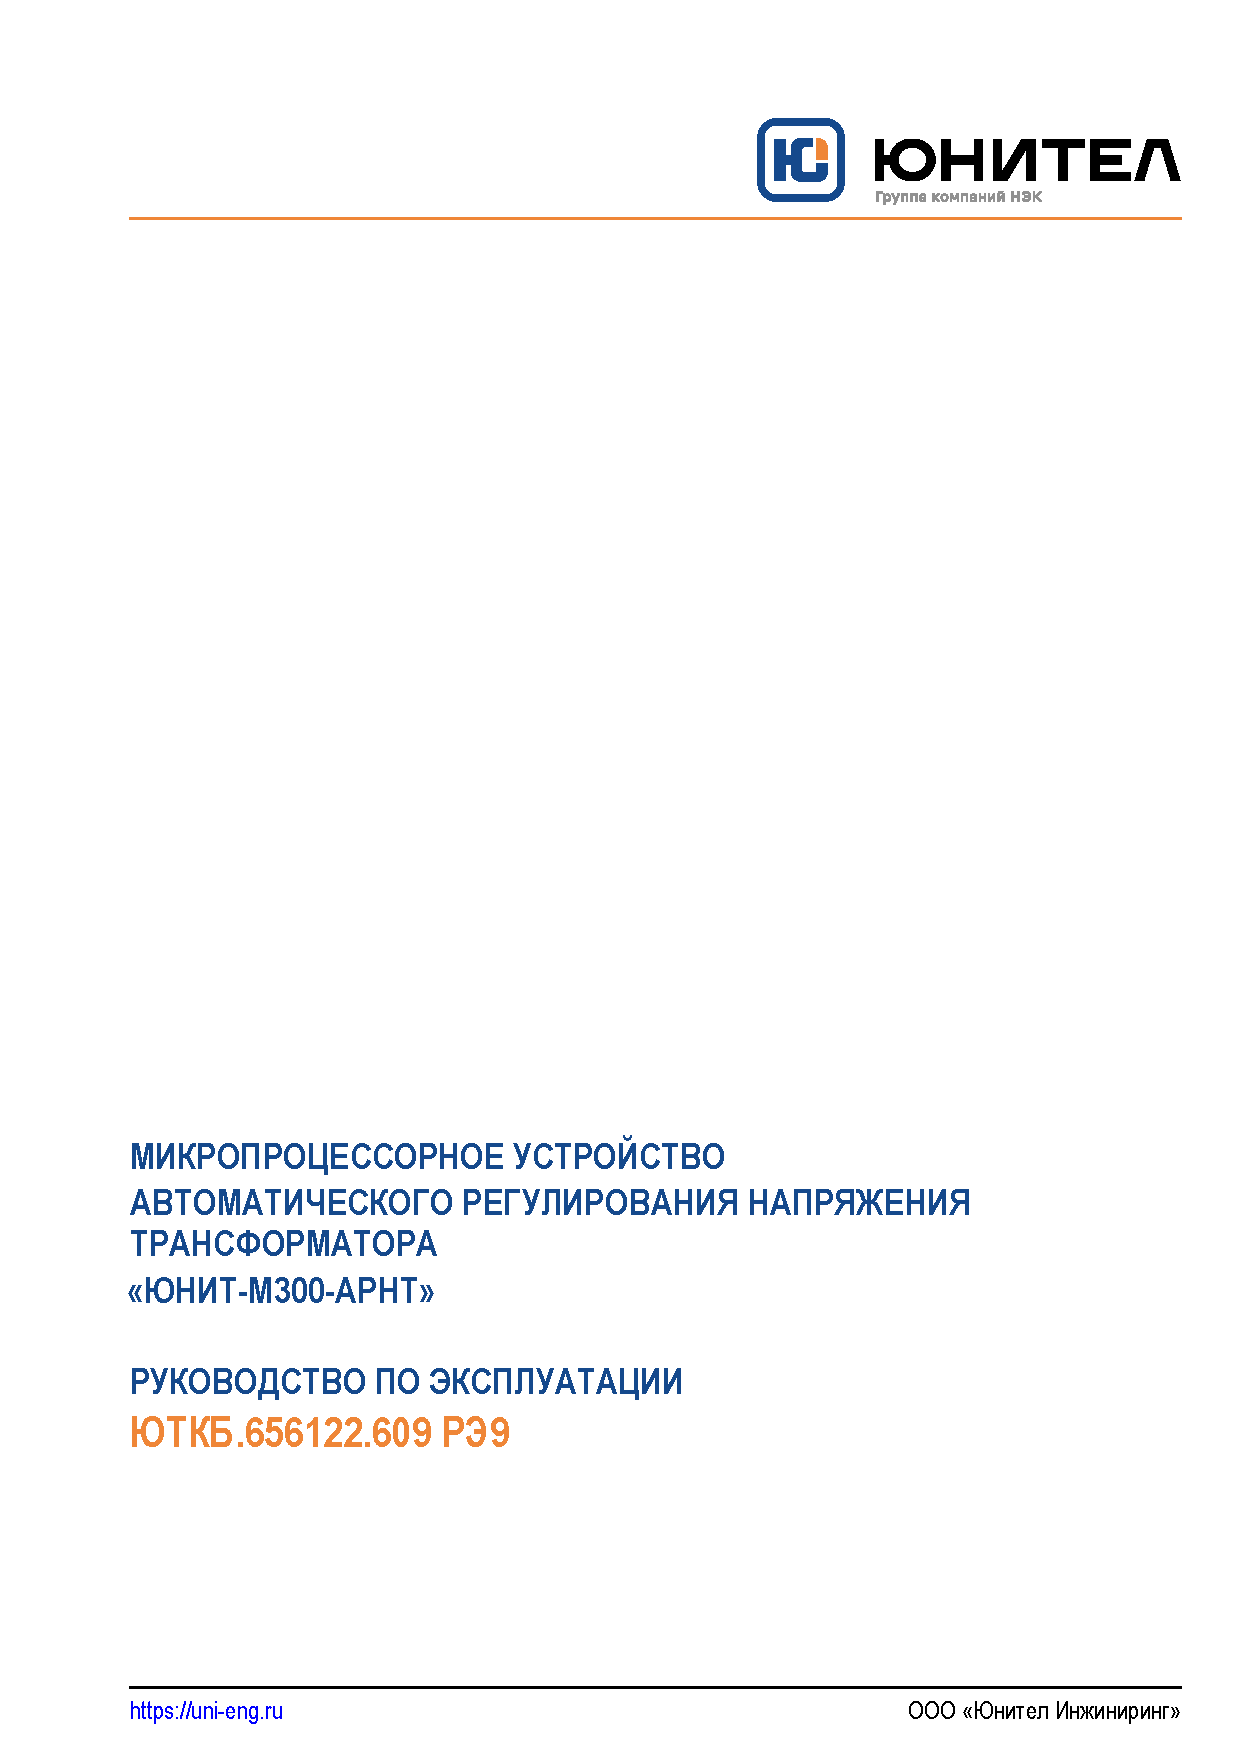
\includepdf[pages={1},width=0.5\textwidth, angle=90]{1.pdf} вставляем и поворачиваем pdf
%\begin{center}
%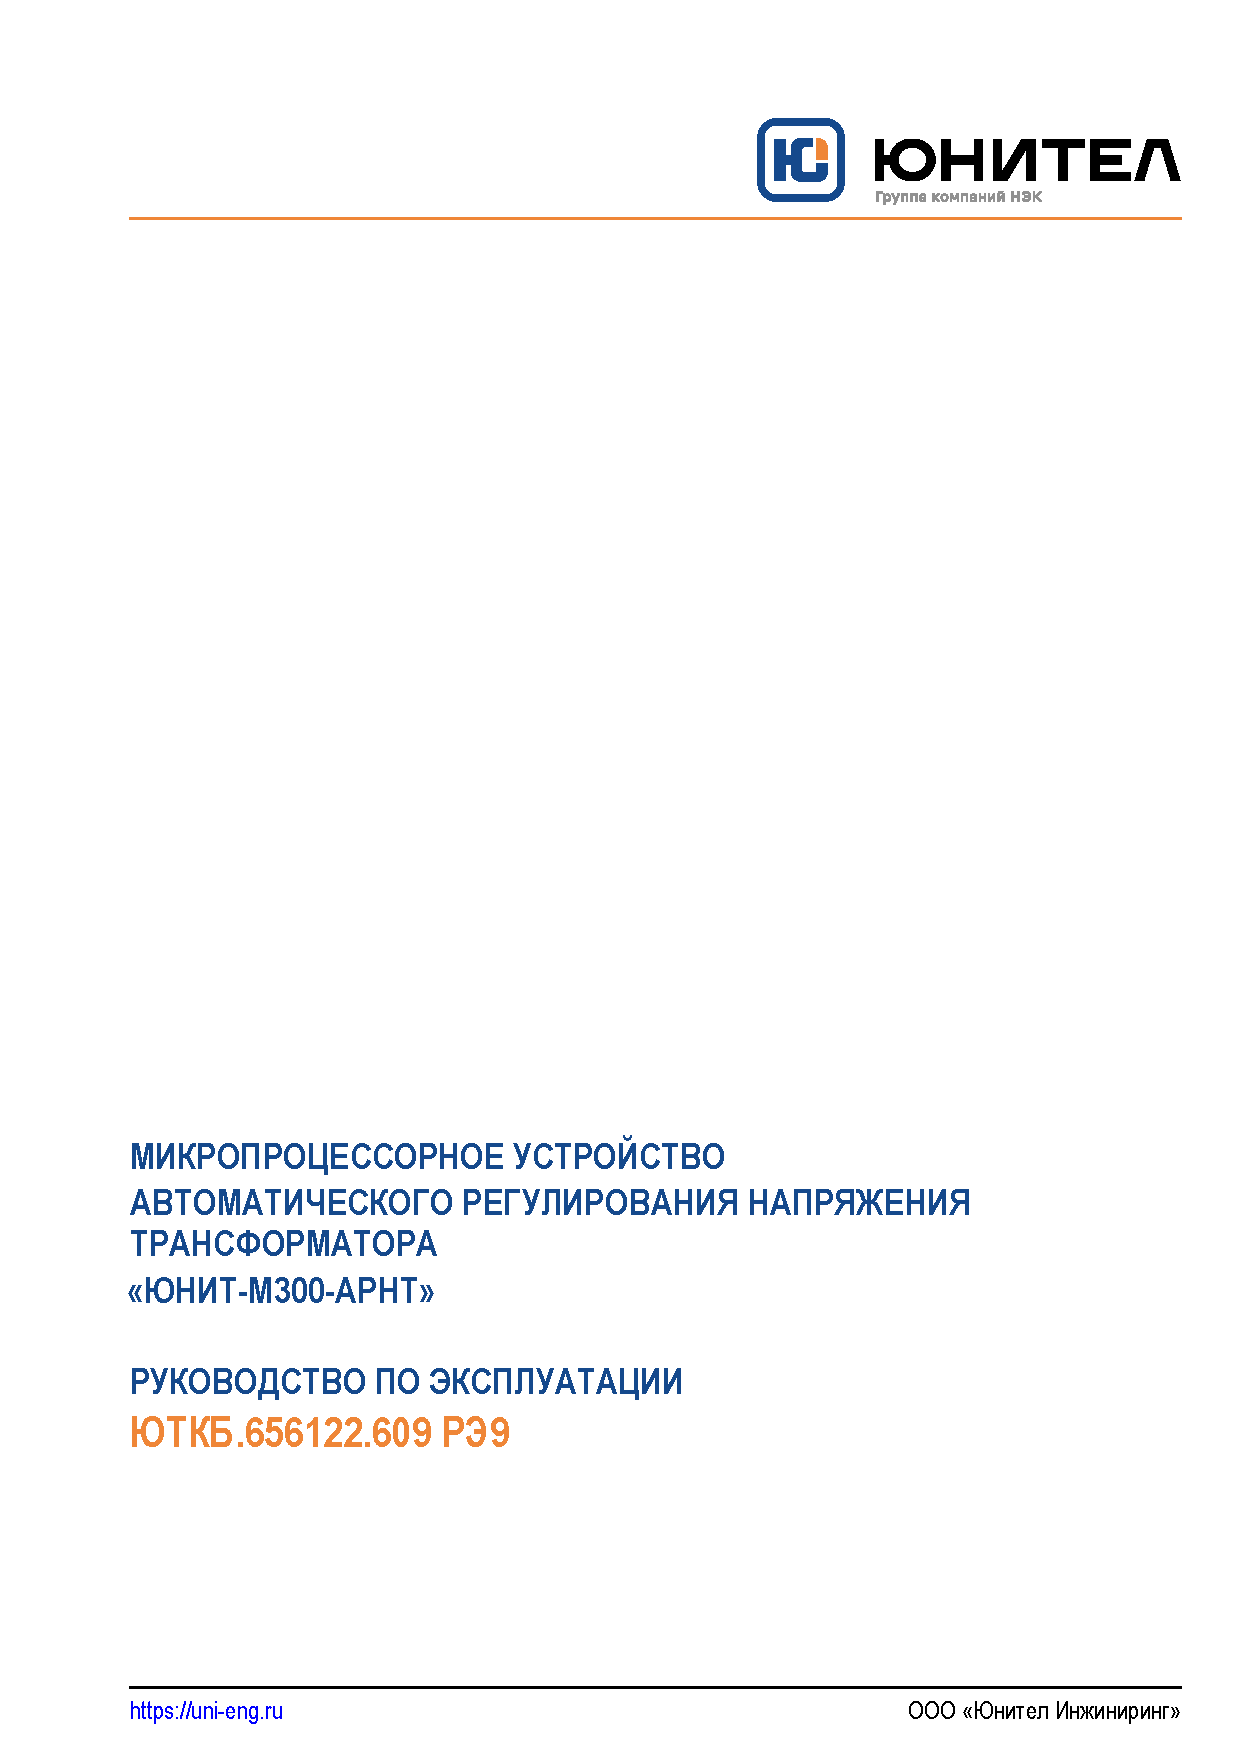
\includegraphics[width=1.4\textwidth]{1.pdf}
%\end{center}

\end{landscape}
\restoregeometry
